\documentclass[aspectratio=169]{beamer}
\usepackage{graphicx}
\usepackage{overpic}
\usepackage{amsmath}
\usepackage[style=vancouver]{biblatex}
\addbibresource{citation.bib}
\usetheme{Madrid}
\usecolortheme{default}
\title[Highlights]{Particle Based Fluid Simulation Using Smoothed Particles Hydrodynamics (SPH)}
\author{Law Chun Man}
\institute{PHYS 4061 Literature Review}
\date{\today}
\setbeamertemplate{footline}{}
\setbeamertemplate{navigation symbols}{}
\setbeamertemplate{caption}{\insertcaption}





\begin{document}
\frame{\titlepage}





\begin{frame}
\frametitle{Literature}


\begin{columns}
\begin{column}{0.45\textwidth}
\begin{figure}
    \centering
    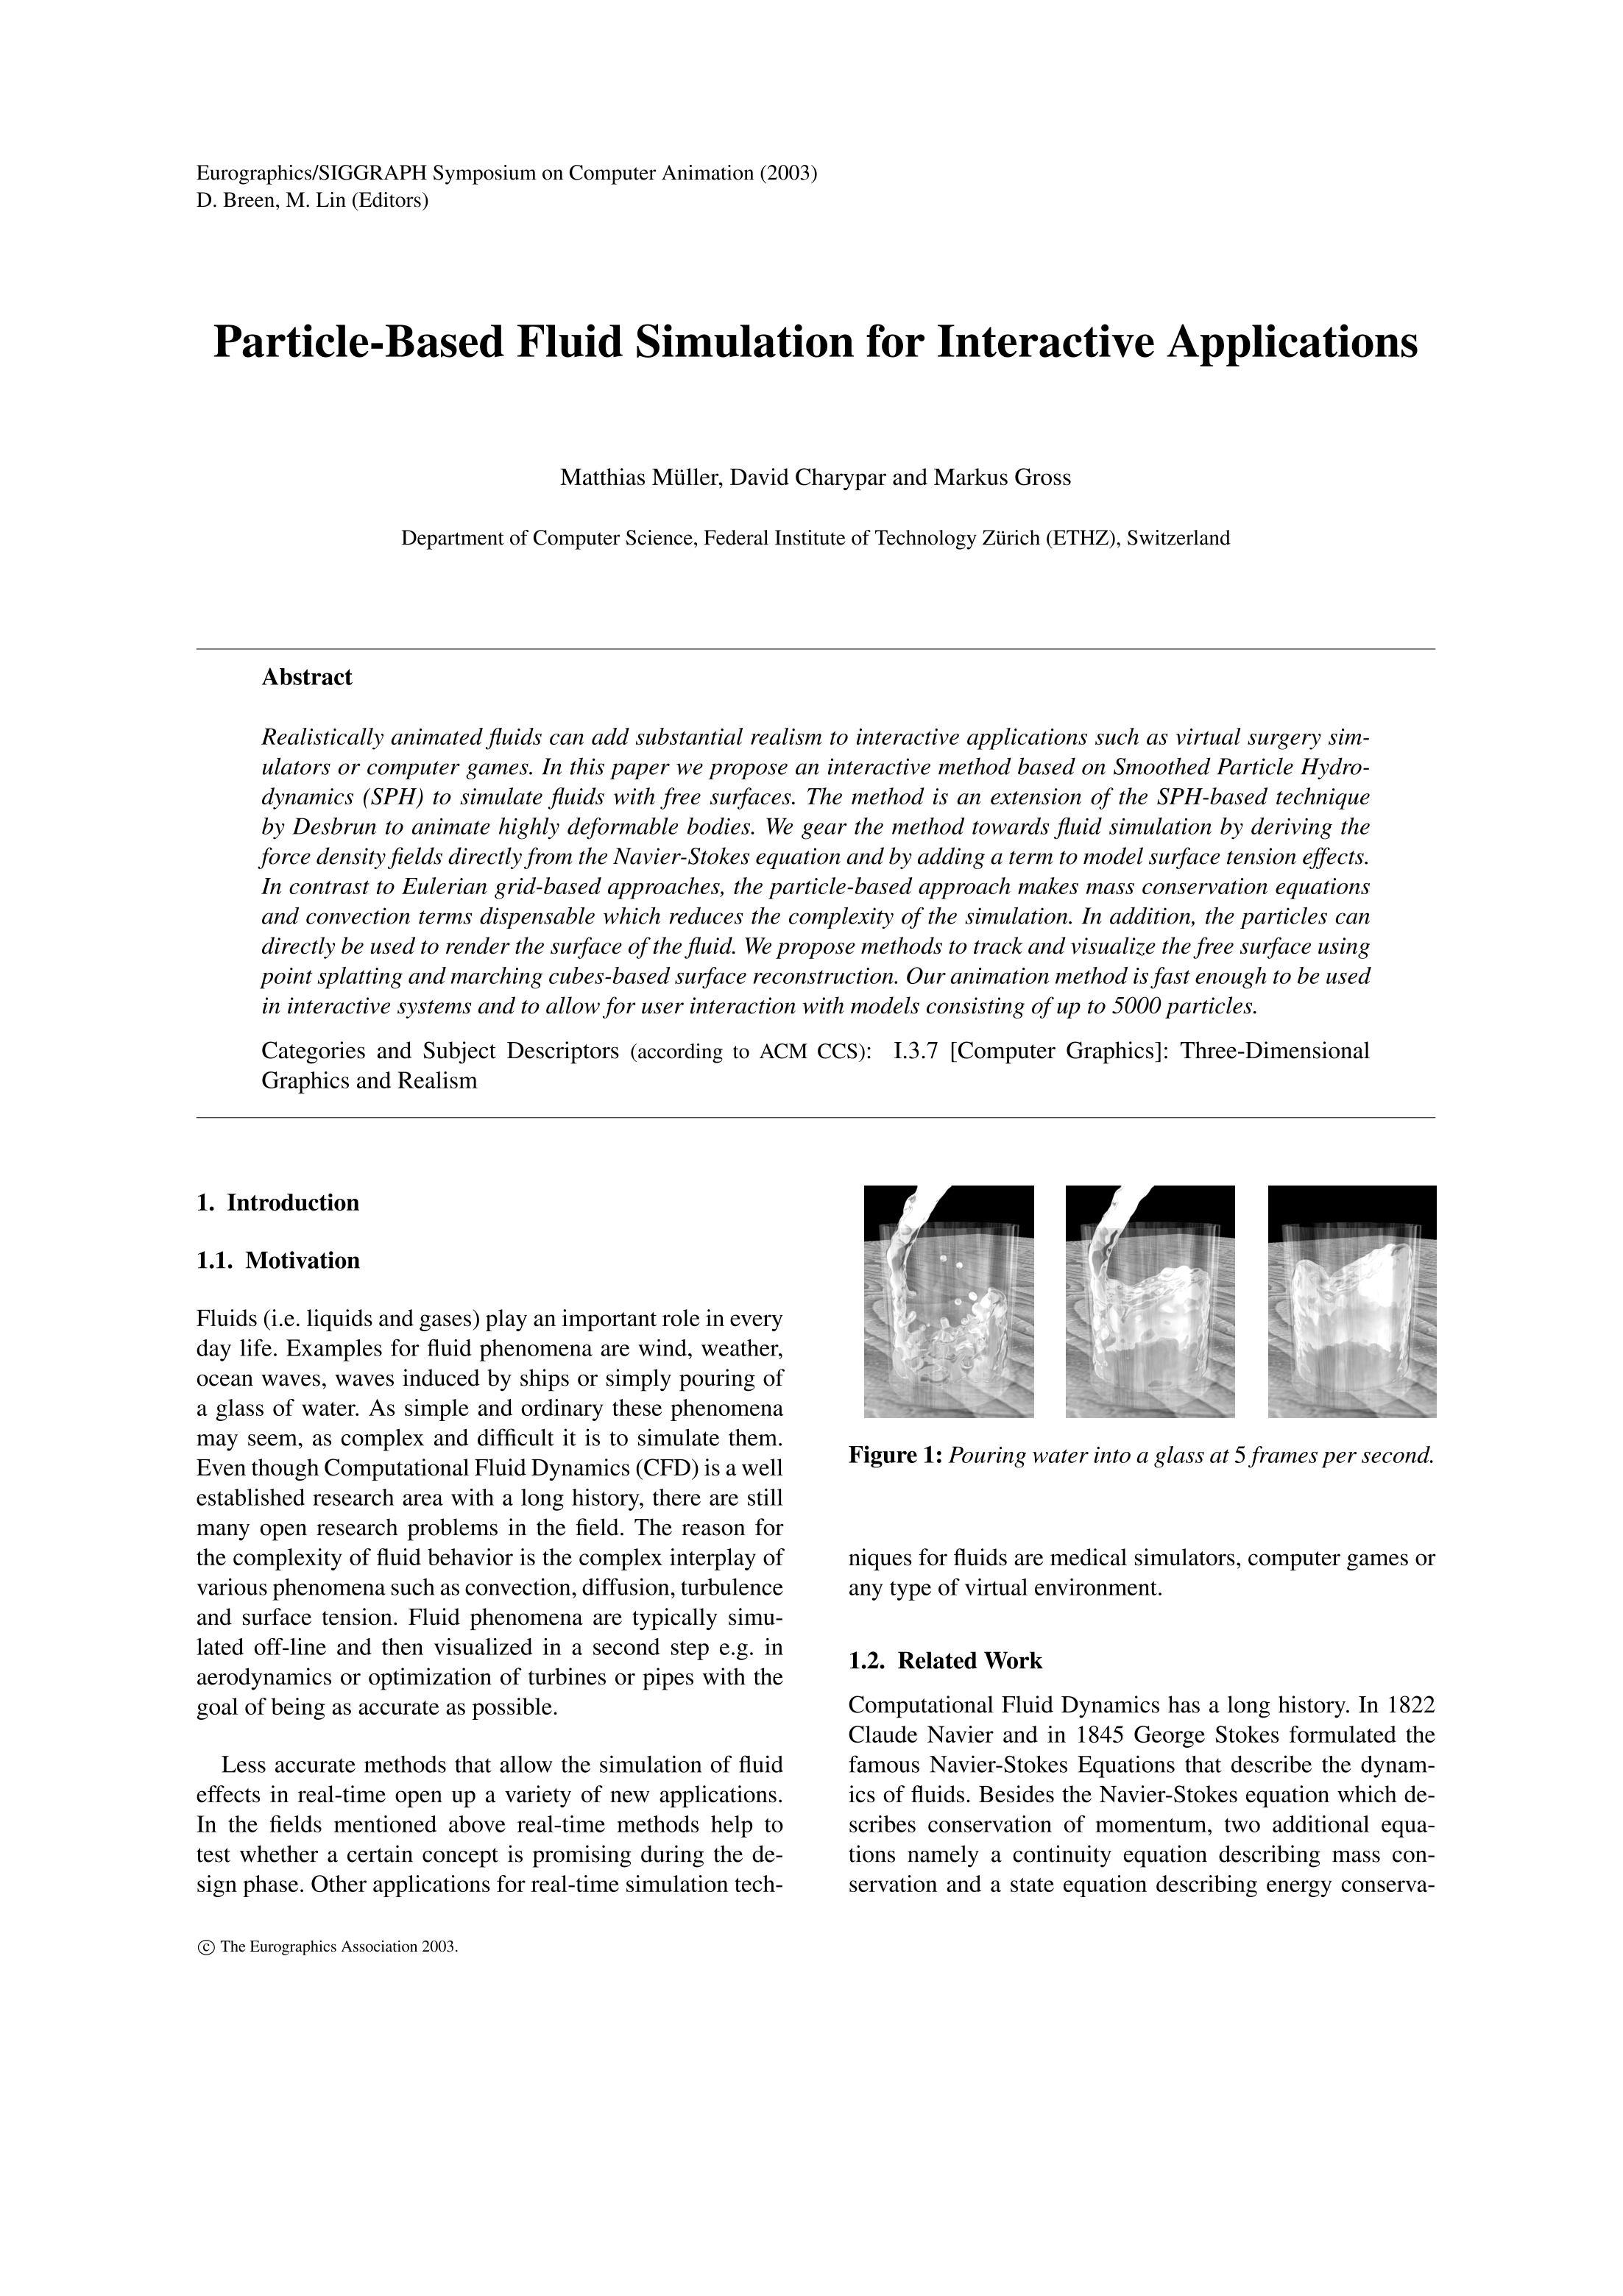
\includegraphics[width=0.6\textwidth]{pictures/paper_thumbnail.png}
    \caption{Particle-Based Fluid Simulation for Interactive Applications~\cite{muller2003particle}}
\end{figure}
\end{column}


\begin{column}{0.45\textwidth}
\begin{figure}
    \centering
    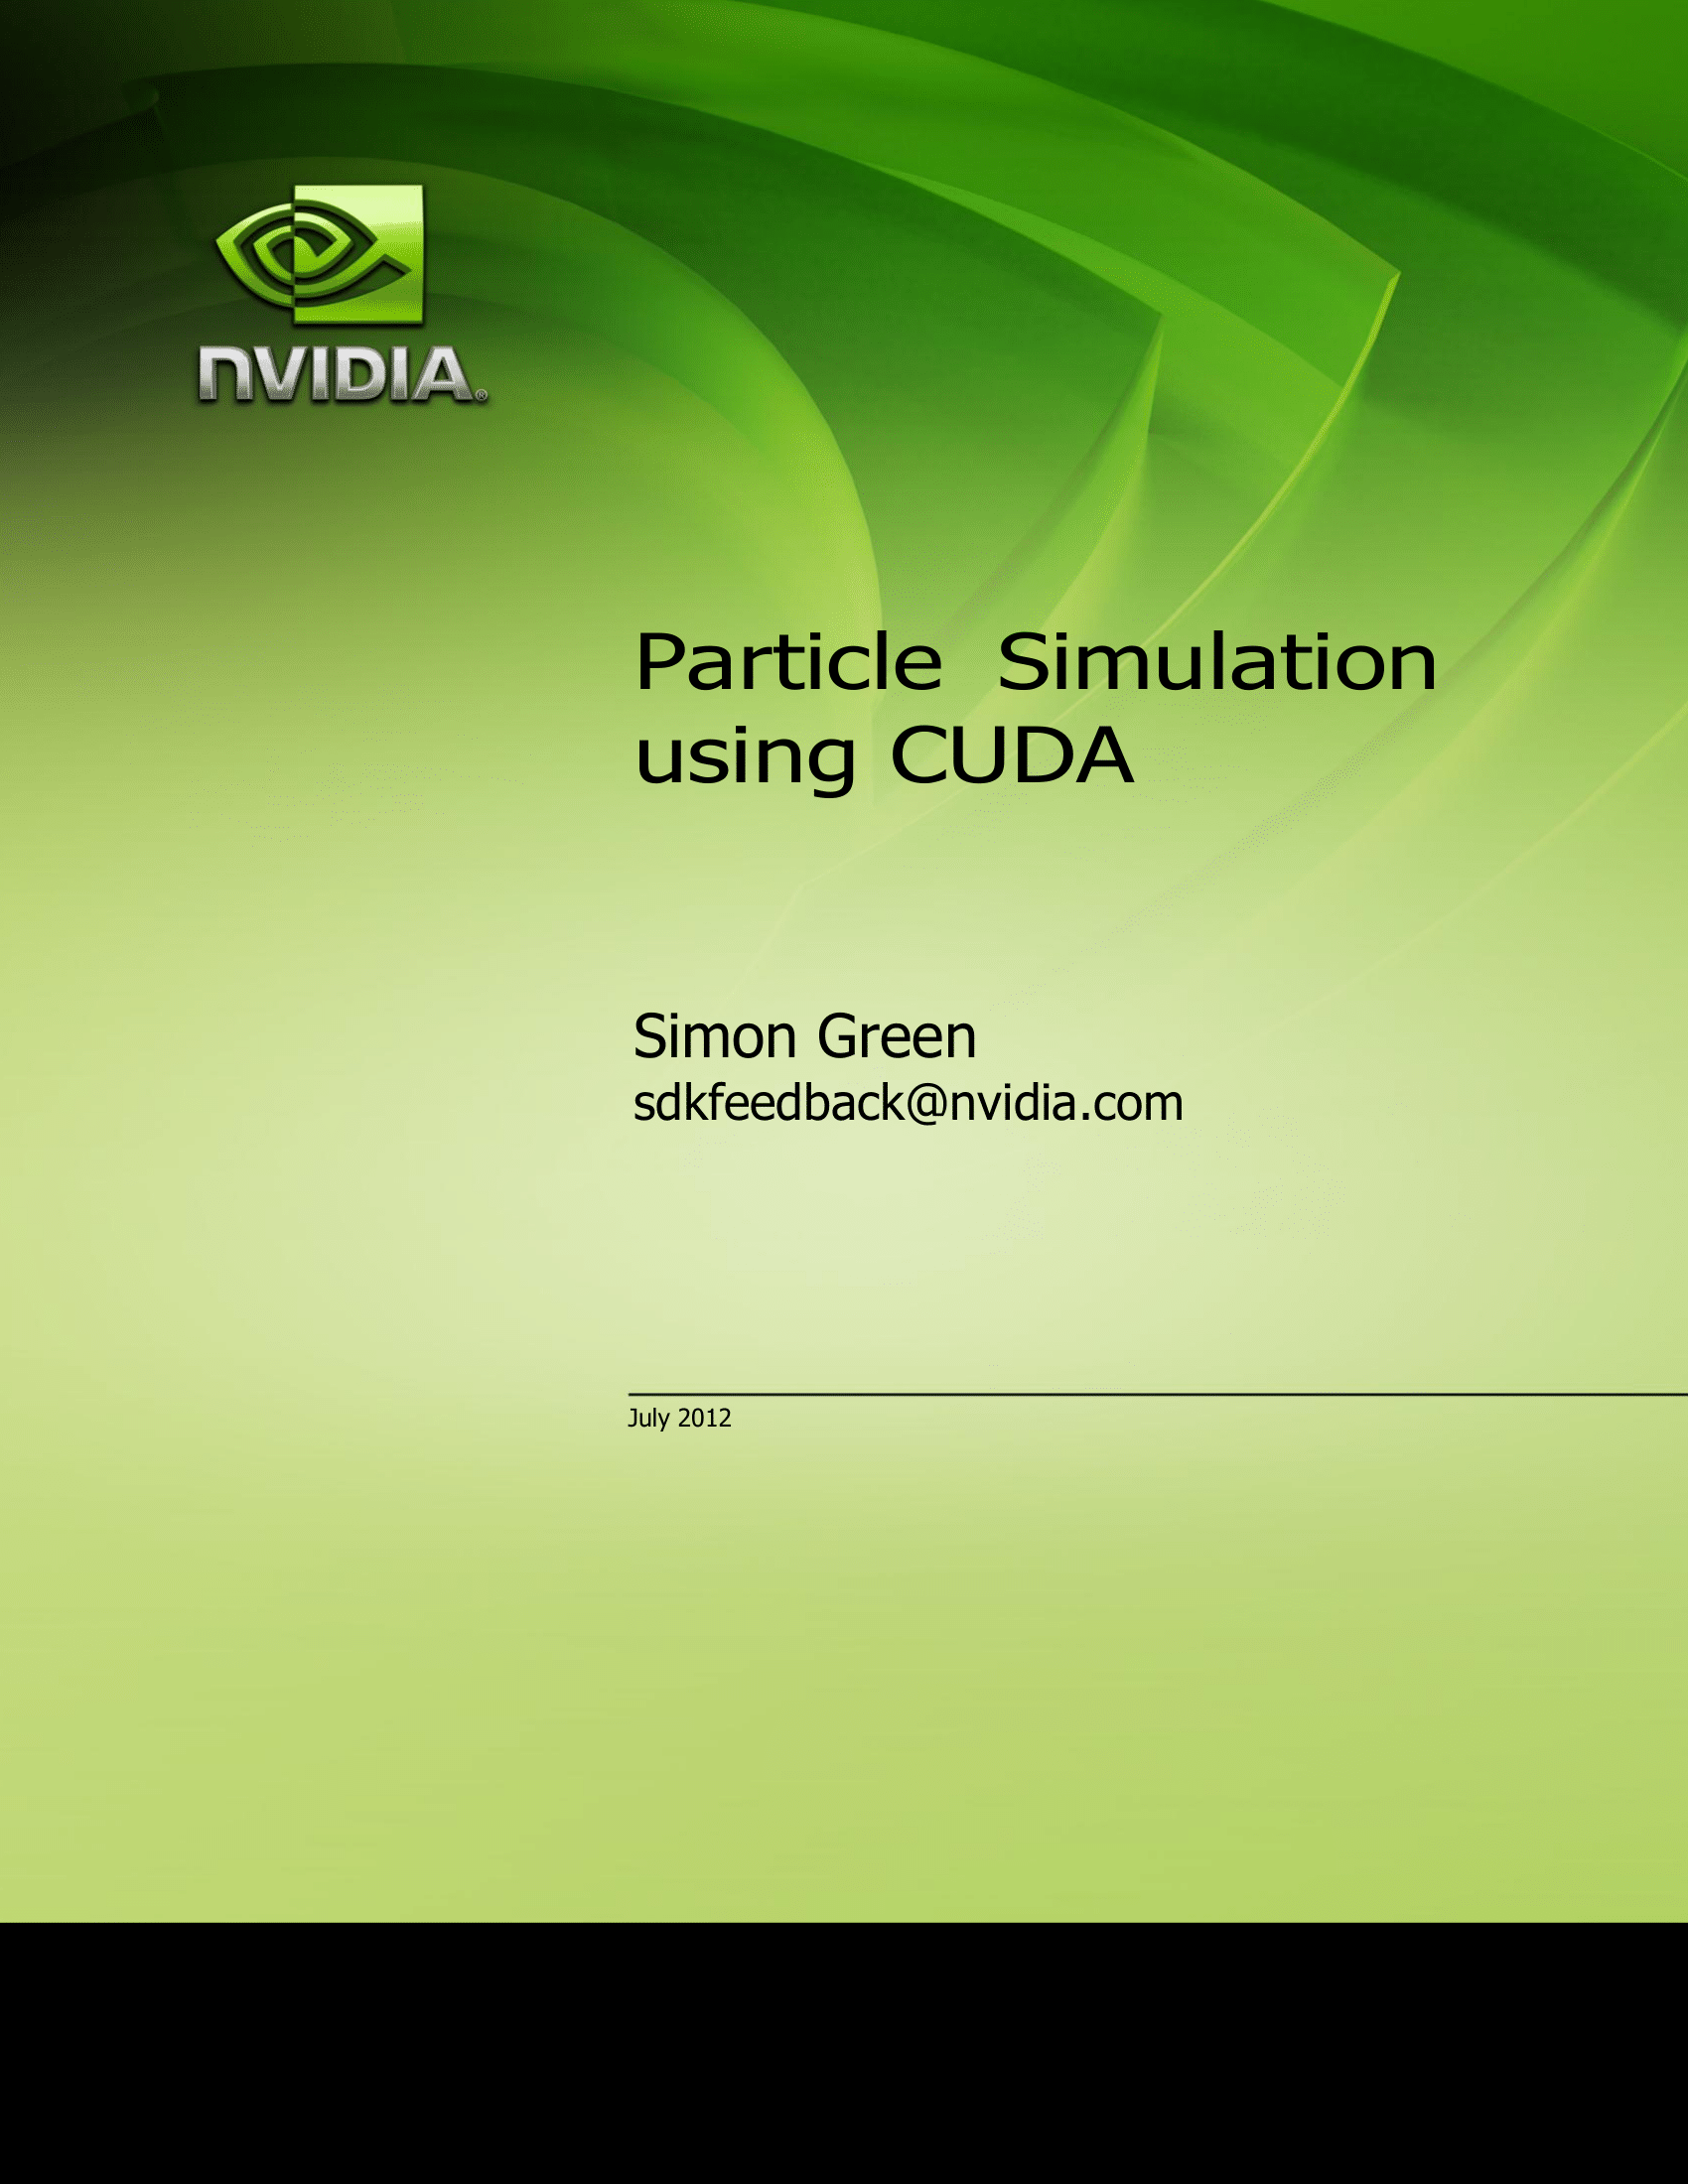
\includegraphics[width=0.6\textwidth]{pictures/paper_thumbnail2.png}
    \caption{Particle Simulation using CUDA~\cite{green2010particle}}
\end{figure}
\end{column}
\end{columns}


\end{frame}





\begin{frame}
\frametitle{Why Smoothed Particles Hydrodynamics}
\begin{block}{Goal}
To realistically animate fluids (water) for interactive applications.
\end{block}
\begin{block}{History}
Smoothed particles hydrodynamics is a numerical technique introduced in 1977 to test the hypothesis that fission is the mechanism by which clone binaries are formed.~\cite{lucy1977numerical}
\end{block}
\begin{block}{Similarities}
Both are based on many particles!
\end{block}
\end{frame}





\begin{frame}
\frametitle{What It Does}
\begin{itemize}
\item Make it more continuous rather than individual particles
\item Better simulate reality with limited number of particles
\end{itemize}


\begin{columns}
\begin{column}{0.32\textwidth}
\begin{figure}

\includegraphics[width=0.9\textwidth]{pictures/particles.png}
\end{figure}
\end{column}

\begin{column}{0.32\textwidth}
\begin{figure}

\includegraphics[width=0.9\textwidth]{pictures/smoothed_particles_5.png}
\end{figure}
\end{column}

\begin{column}{0.32\textwidth}
\begin{figure}

\includegraphics[width=0.9\textwidth]{pictures/smoothed_particles_10.png}
\end{figure}
\end{column}
\end{columns}
\end{frame}





\begin{frame}
\frametitle{Modeling Equations}
\begin{block}{Conservation of mass}
\[
\frac{\partial \rho}{\partial t}+\nabla\cdot\left(\rho\mathbf{v}\right)=0,
\]
\end{block}
where \(\rho\) is the density, \(\mathbf{v}\) is the velocity field.
\begin{block}{Conservation of momentum}
\[
\rho\left(\frac{\partial \mathbf{v}}{\partial t}\right) = -\nabla p + \rho \mathbf{g} + \mu \nabla^2 \mathbf{v},
\]
\end{block}
where \(p\) is the pressure field, \(\mathbf{g}\) is the external force density, \(\mu\) is the viscosity of the fluid.
\end{frame}





\begin{frame}
\frametitle{Interpolating Equation}
\only<1>{
\[
A_S\left(\mathbf{r}\right)=\sum_j m_j \frac{A_j}{\rho_j} W\left(\mathbf{r}-\mathbf{r}_j, h\right)\text{,}
\]
where \(A\) is some physical quantities, \(m\) is the mass of particle, \(\mathbf{r}\) is the position of particle, \(\rho\) is the density, and \(W\left(\mathbf{r}, h\right)\) is the smoothing kernel with core radius h.

\begin{block}{Density}
\vspace{-1em}
\begin{align*}
\rho\left(\mathbf{r}\right)&=\sum_j m_j \frac{\rho_j}{\rho_j}W\left(\mathbf{r}_i-\mathbf{r}_j, h\right), \\
\rho\left(\mathbf{r}\right)&=\sum_j m_j W\left(\mathbf{r}_i-\mathbf{r}_j, h\right),
\end{align*}
\end{block}
}

%\only<2>{
%\begin{block}{Pressure}
%\vspace{-1em}
%\begin{align*}
%\mathbf{f}_i^{\text{pressure}}&=-\nabla p\left(\mathbf{r}_i\right) = -\sum_j m_j \frac{p_j}{\rho_j}\nabla W\left(\mathbf{r}_i-\mathbf{r}_j, h\right), \\
%\mathbf{f}_i^{\text{pressure}} &= -\sum_j m_j \frac{p_i+p_j}{2\rho_j}\nabla W\left(\mathbf{r}_i-\mathbf{r}_j, h\right),
%\end{align*}
%\end{block}
%
%
%\begin{block}{Viscosity}
%\vspace{-1em}
%\begin{align*}
%\mathbf{f}_i^{\text{viscosity}}&=\mu\nabla^2 \mathbf{v}\left(\mathbf{r}_i\right) = \mu\sum_j m_j \frac{\mathbf{v}_j}{\rho_j}\nabla^2 W\left(\mathbf{r}_i-\mathbf{r}_j, h\right), \\
%\mathbf{f}_i^{\text{viscosity}}&= \mu\sum_j m_j \frac{\mathbf{v}_j-\mathbf{v}_i}{\rho_j}\nabla^2 W\left(\mathbf{r}_i-\mathbf{r}_j, h\right),
%\end{align*}
%\end{block}
%where \(\mathbf{f}_i\) is the force density field at the location of particle \(i\).
%}
\end{frame}





\begin{frame}
\frametitle{Smoothing Kernel}
\only<1>{
\begin{itemize}
\item Maximum influence at the centre, no influence for \(\left|\mathbf{r}\right|>h\).
\end{itemize}
\begin{figure}
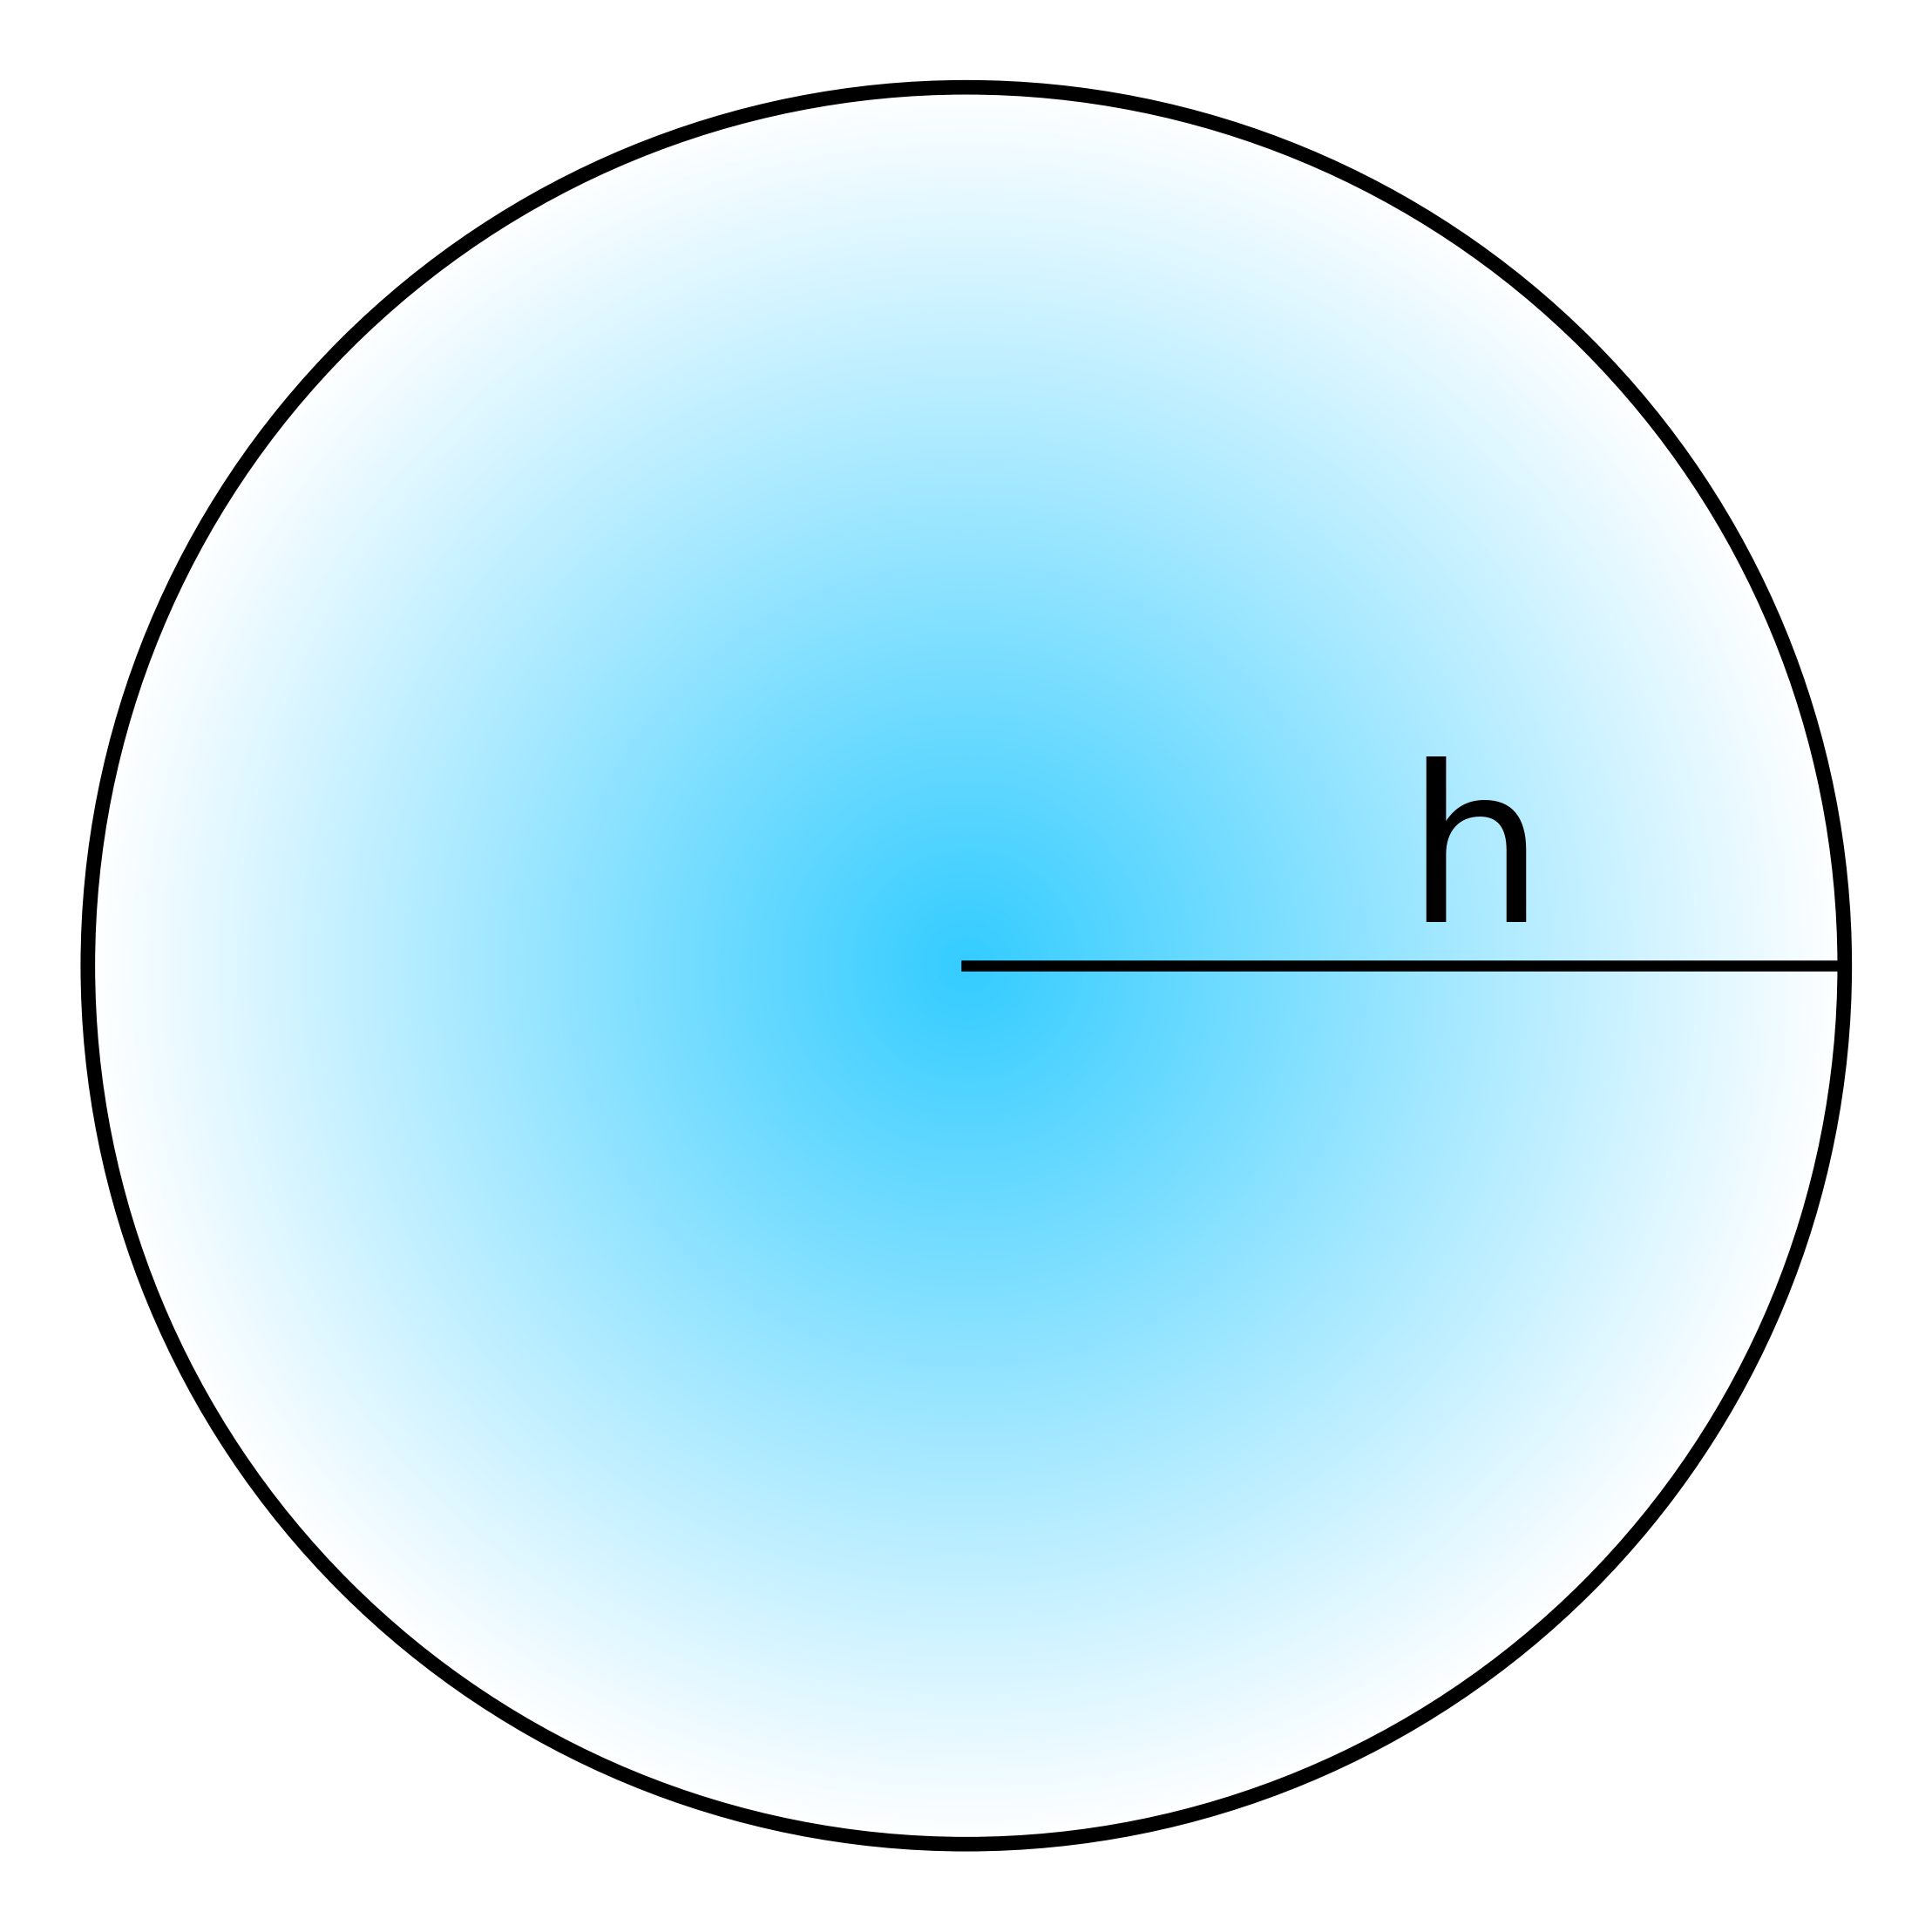
\includegraphics[width=0.4\textwidth]{pictures/smoothing_radius.png}
\end{figure}
}


\only<2->{
\begin{columns}
\begin{column}{0.32\textwidth}
{\scriptsize\[
W\left(\mathbf{r}, h\right) = 
\begin{cases} 
    h-\left|\mathbf{r}\right| & 0 \leq \left|\mathbf{r}\right| \leq h \\ 
    0 & \text{otherwise.}
\end{cases}
\]}
\begin{figure}
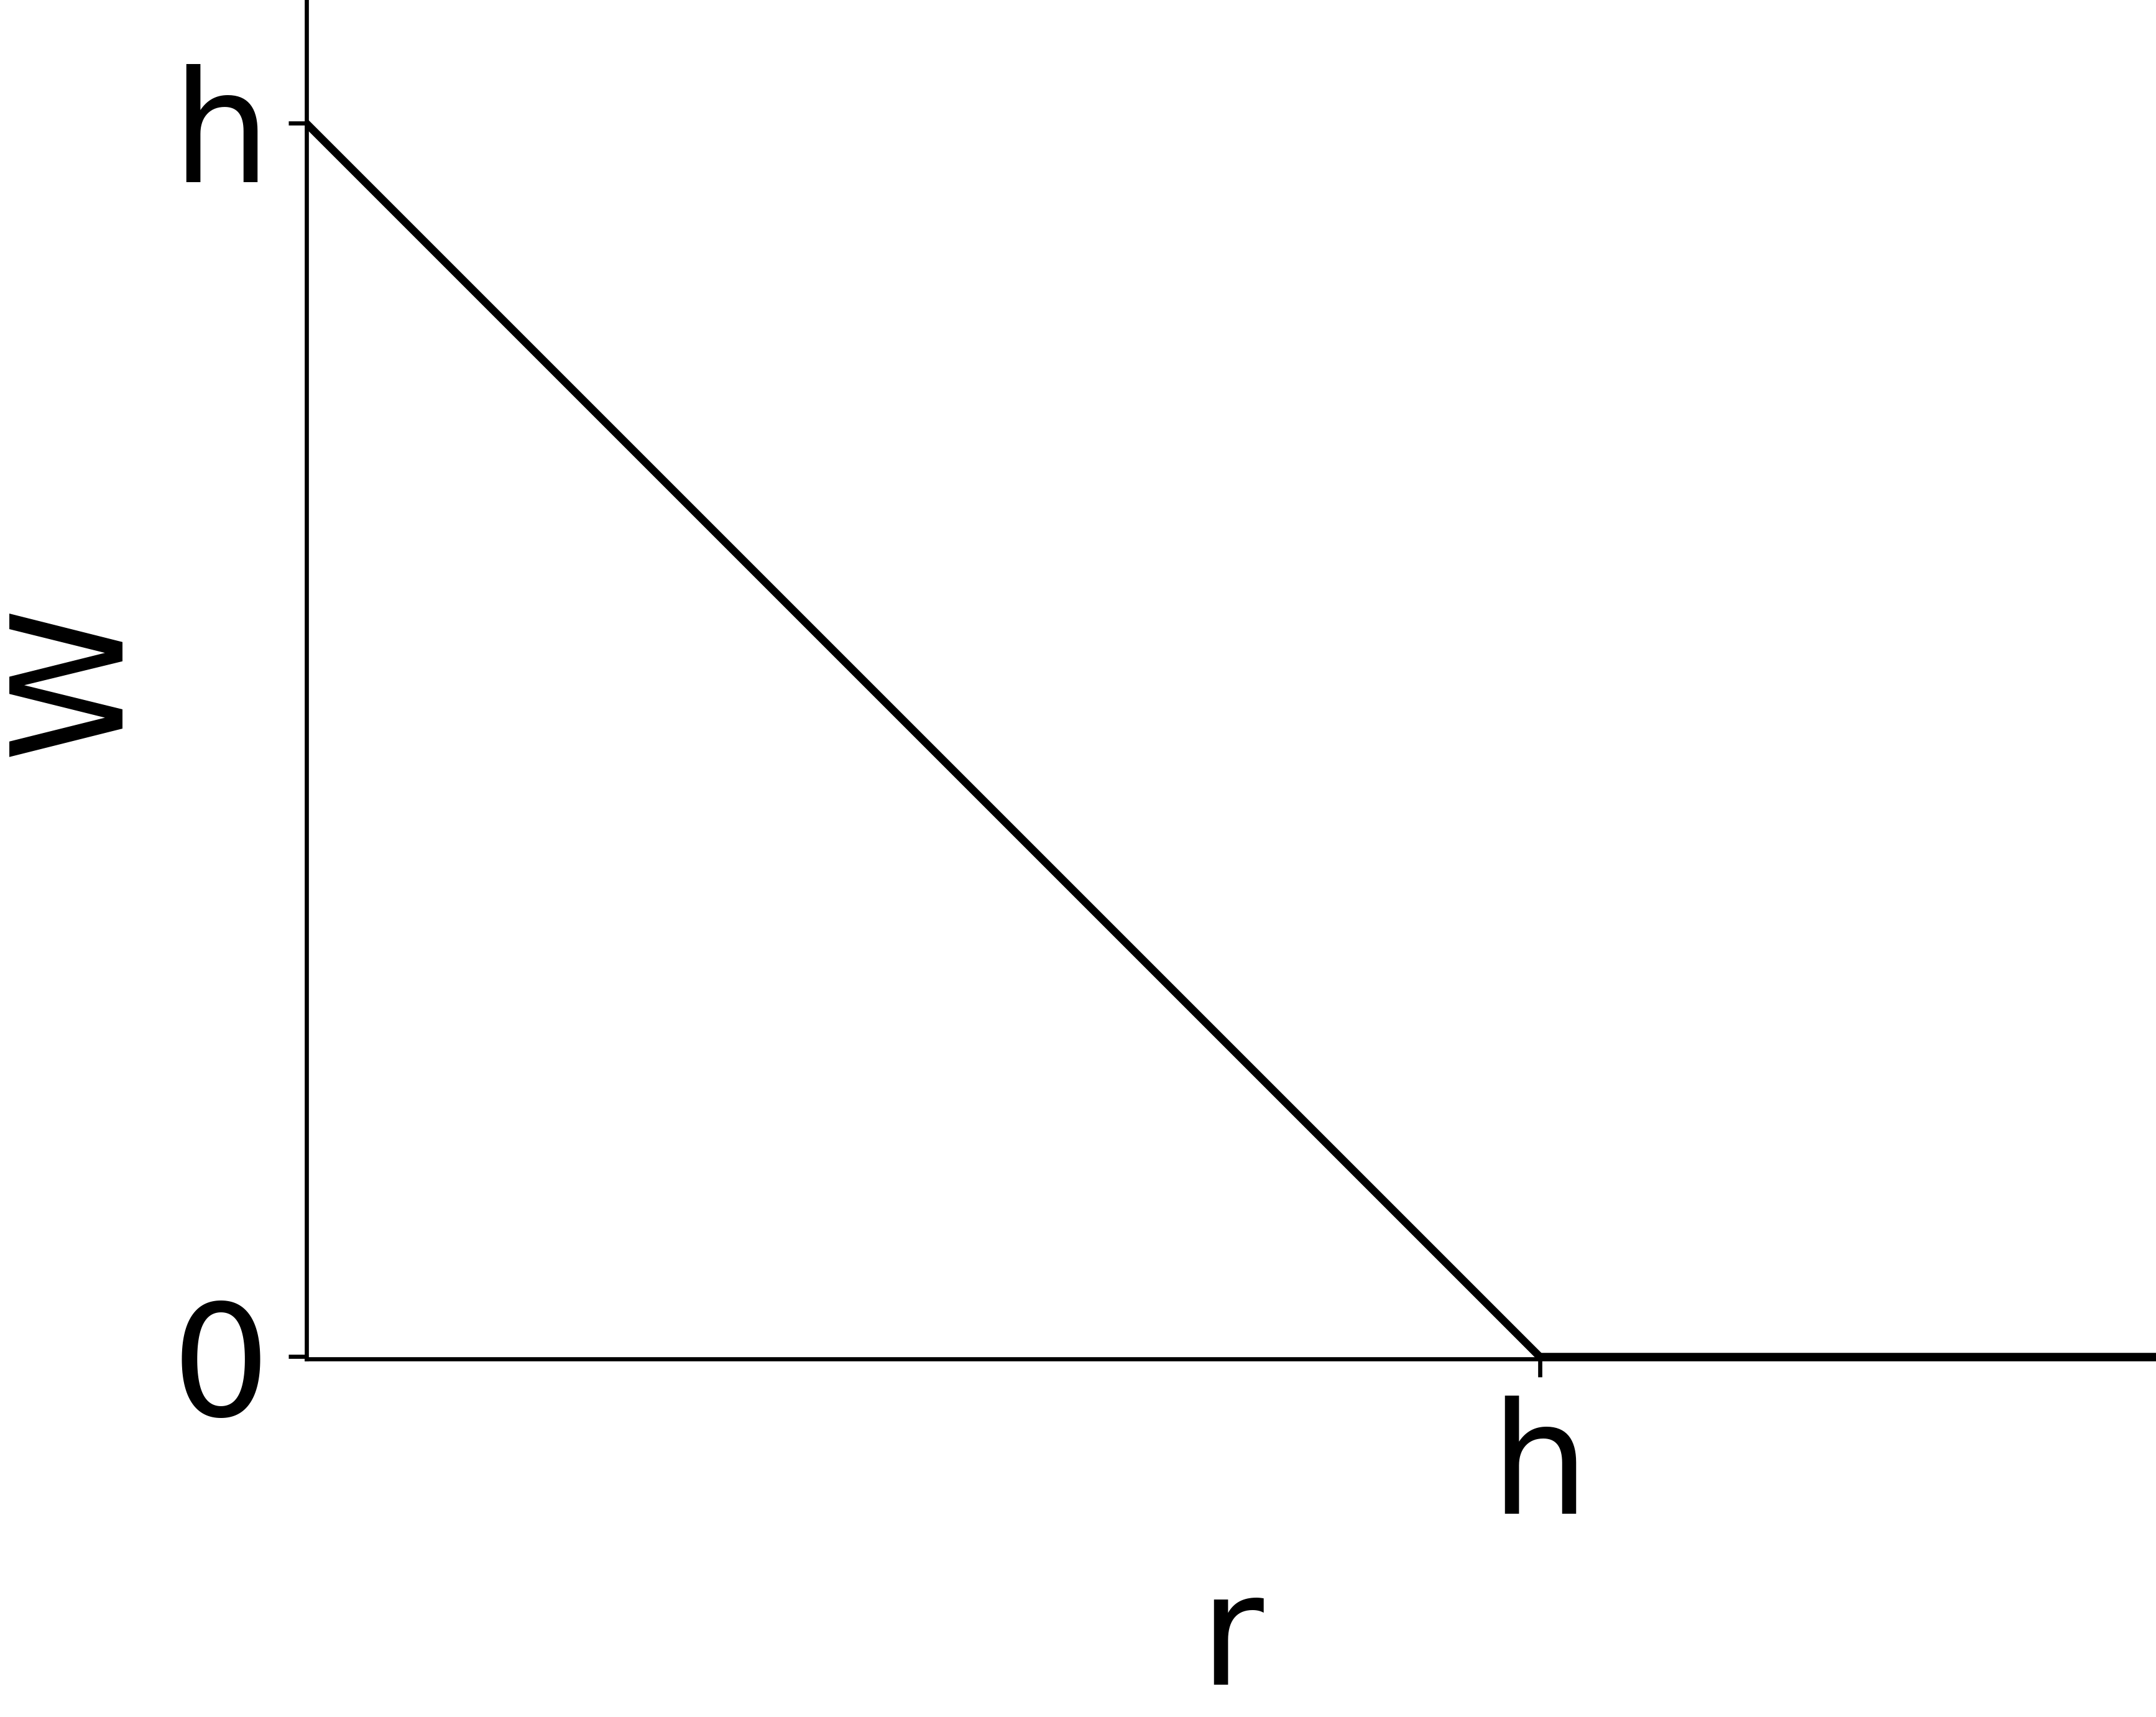
\includegraphics[width=0.9\textwidth]{pictures/smoothing_kernel_1.png}
\end{figure}
\end{column}


\hspace{-1.2em}
\begin{column}{0.32\textwidth}
{\scriptsize\[
W\left(\mathbf{r}, h\right) = 
\begin{cases} 
    \left(h-\left|\mathbf{r}\right|\right)^3 & 0 \leq \left|\mathbf{r}\right| \leq h \\ 
    0 & \text{otherwise.}
\end{cases}
\]}
\begin{figure}
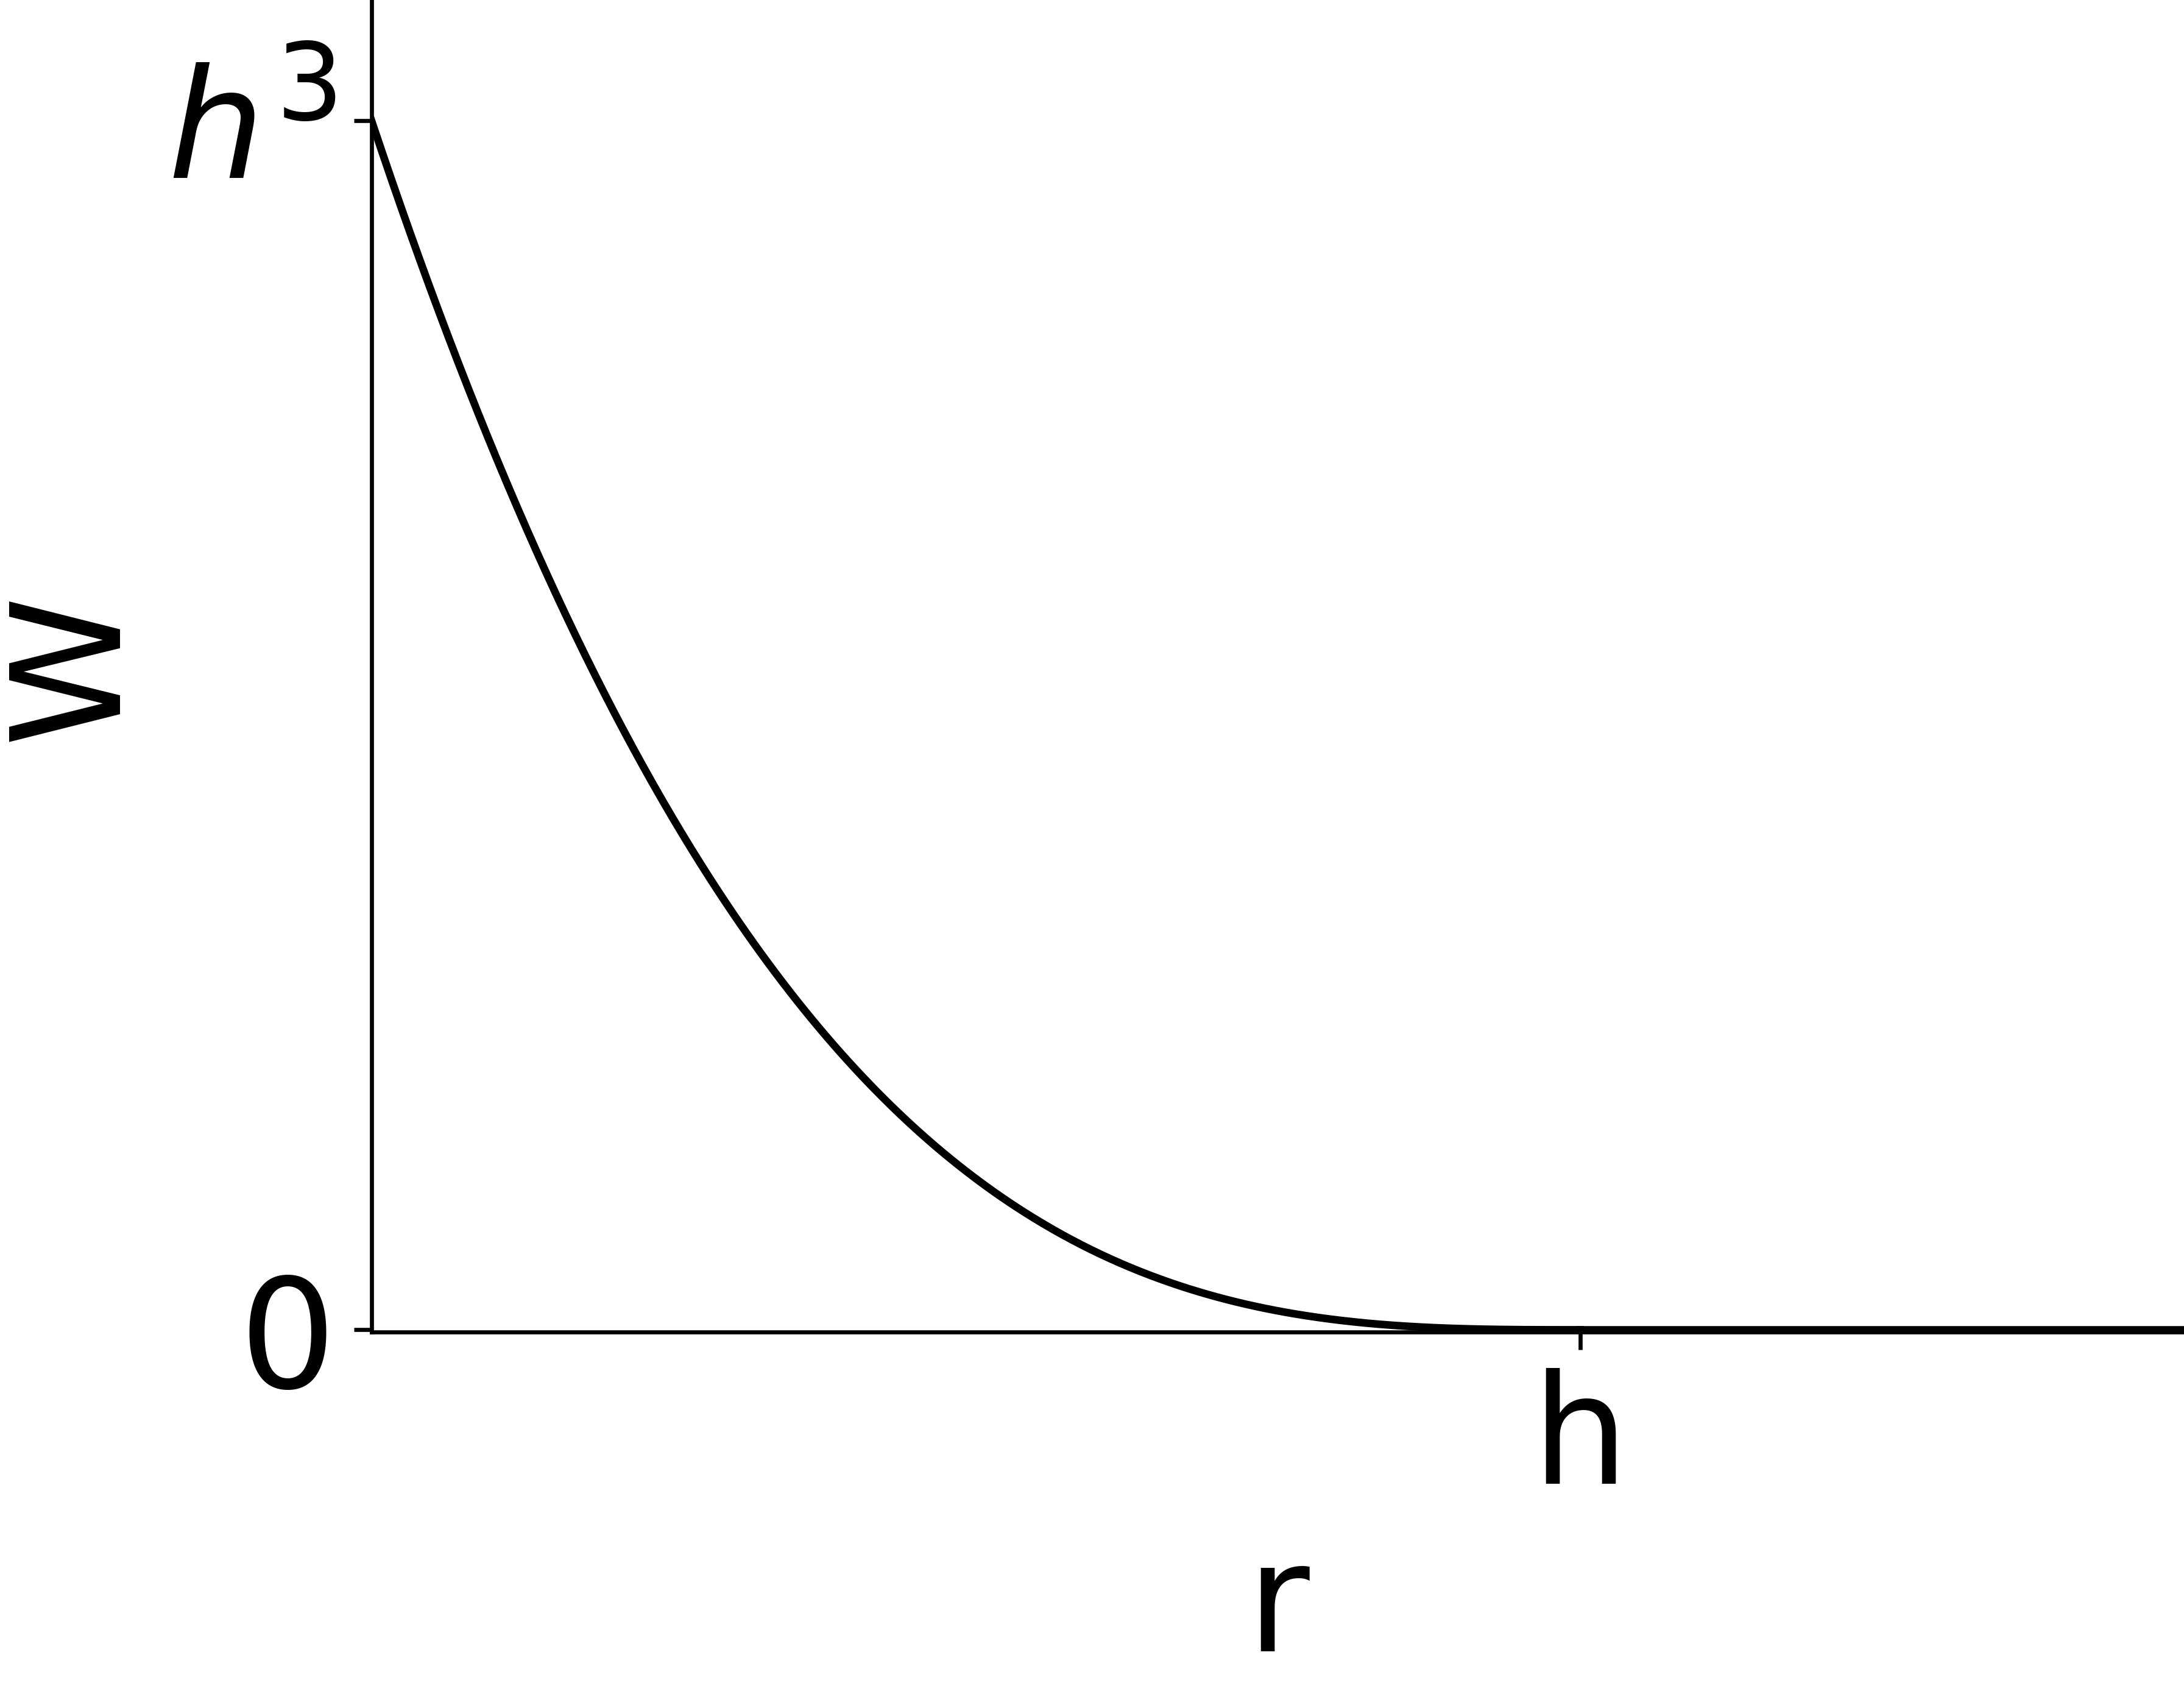
\includegraphics[width=0.9\textwidth]{pictures/smoothing_kernel_2.png}
\end{figure}
\end{column}


\hspace{-1em}
\begin{column}{0.32\textwidth}
{\scriptsize\[
W\left(\mathbf{r}, h\right) = 
\begin{cases} 
    \left(h^2-\left|\mathbf{r}\right|^2\right)^3 & 0 \leq \left|\mathbf{r}\right| \leq h \\ 
    0 & \text{otherwise.}
\end{cases}
\]}
\begin{figure}
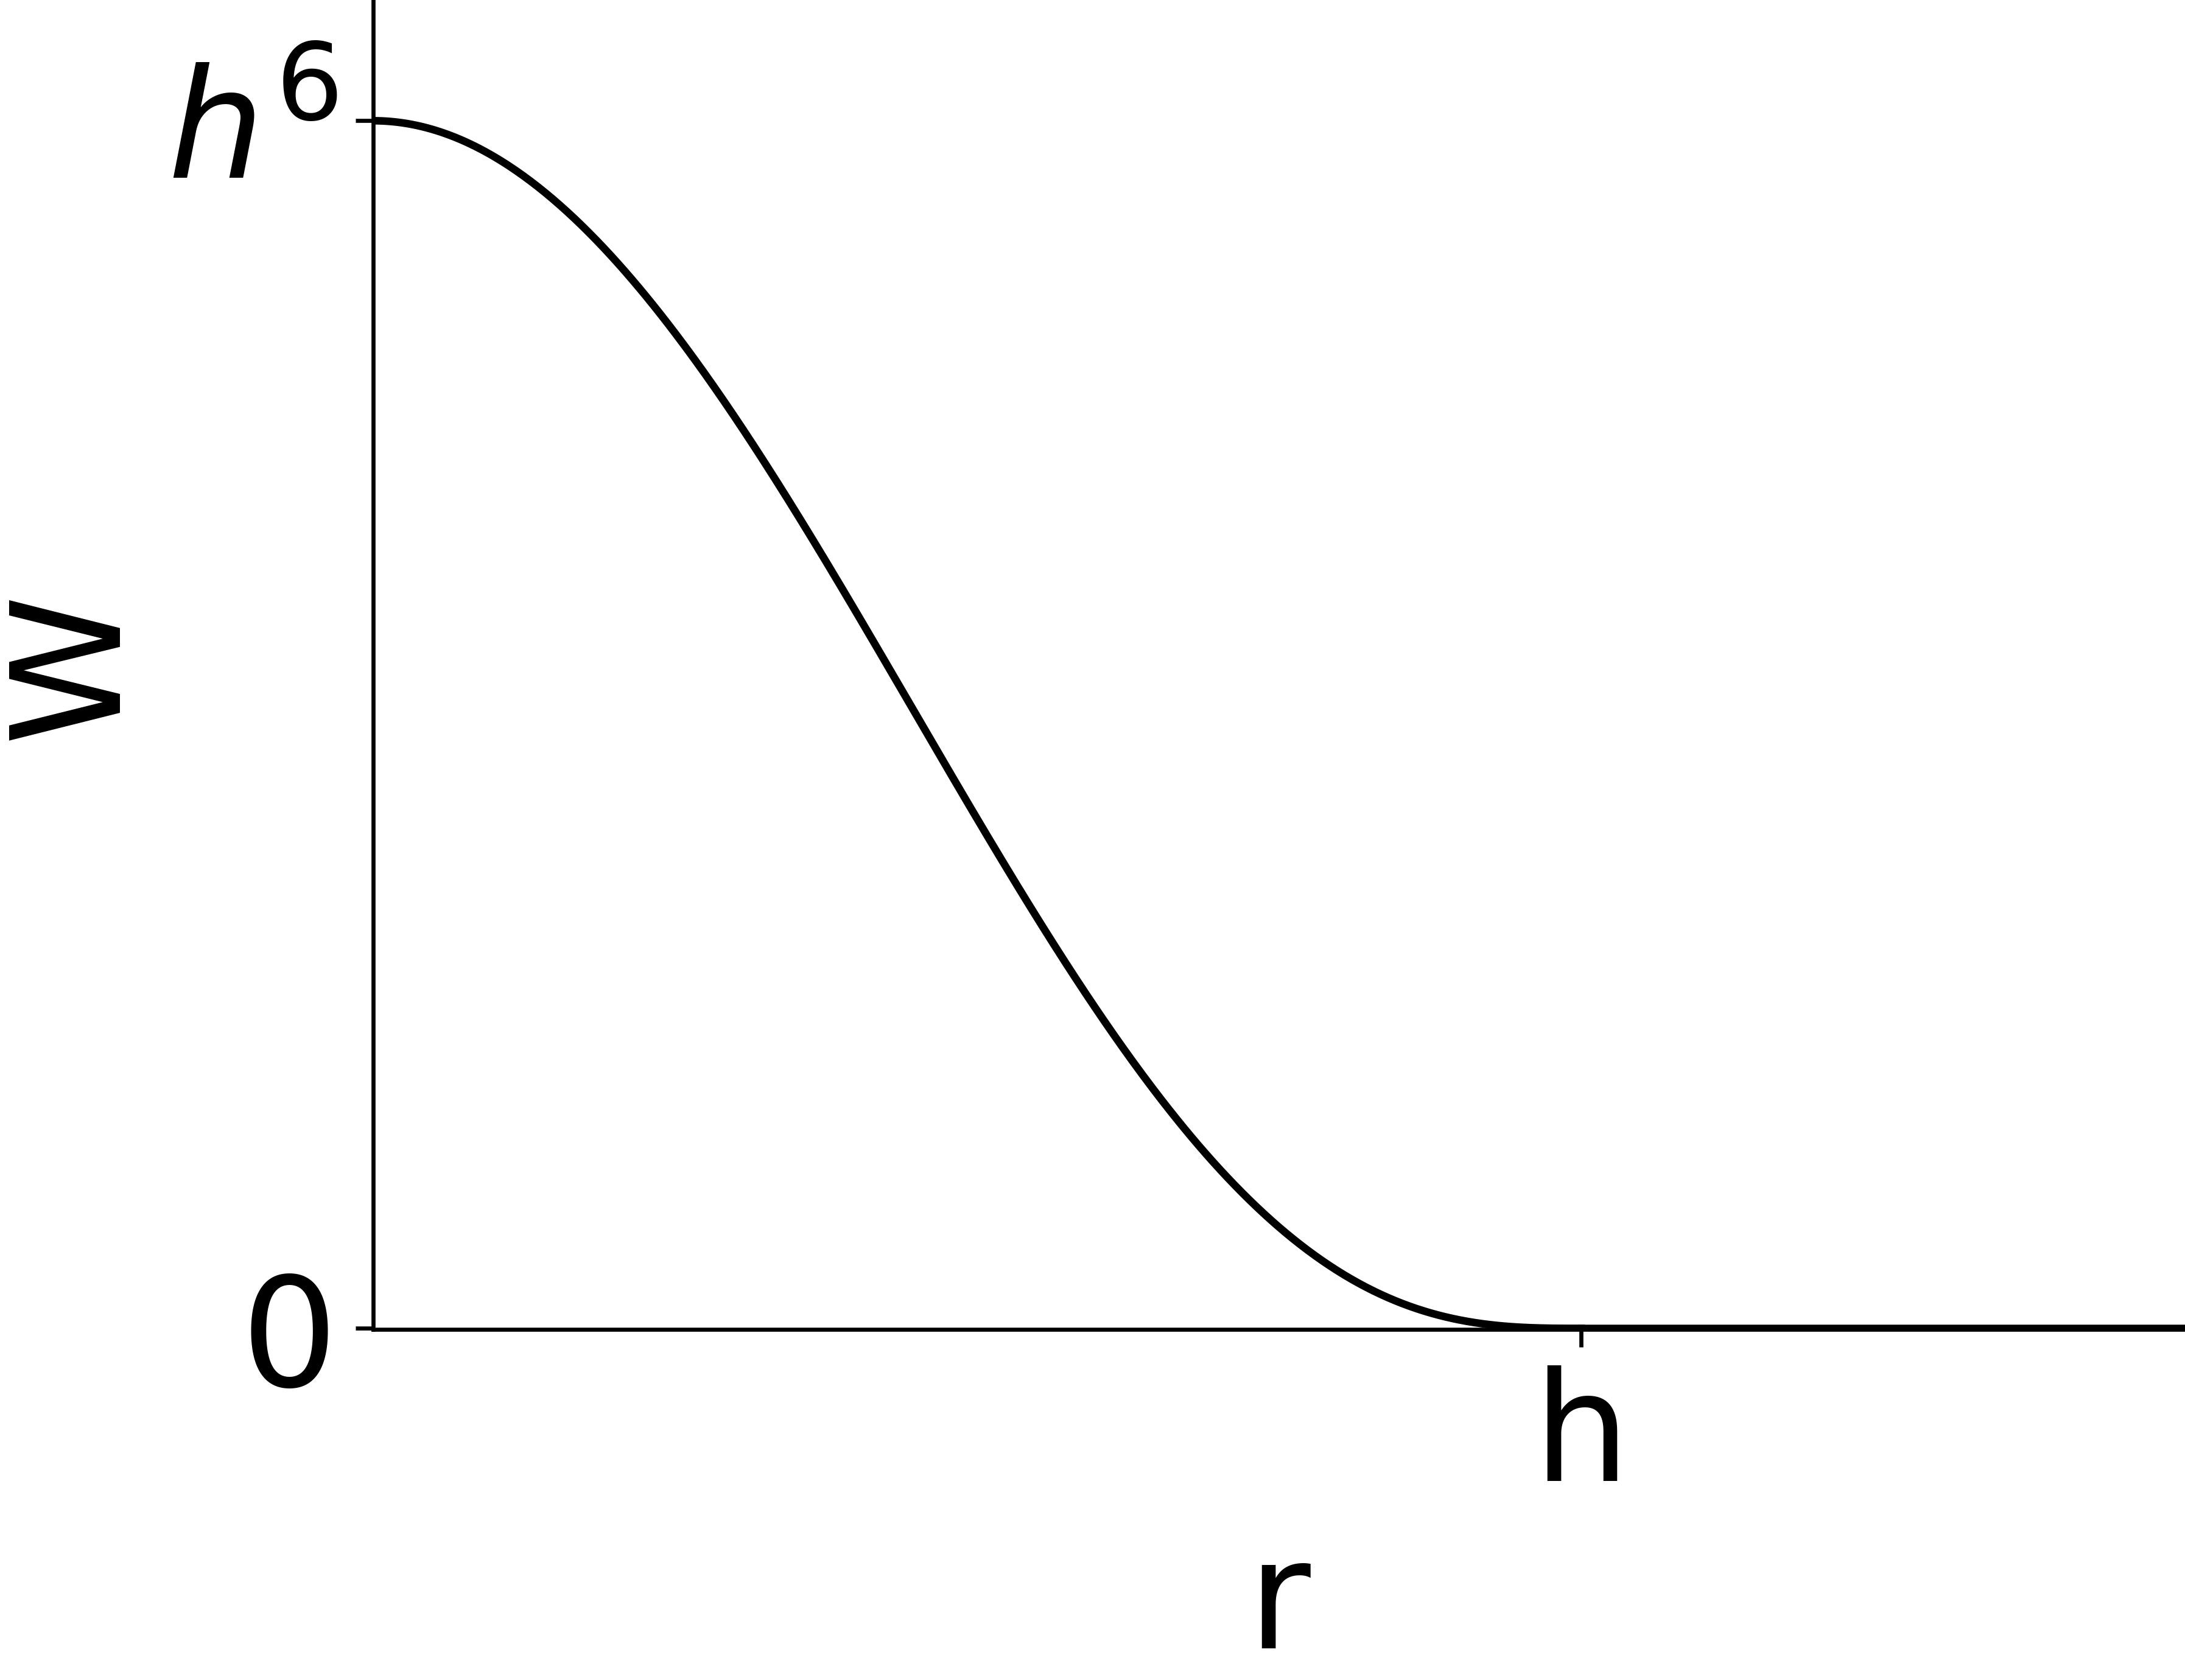
\includegraphics[width=0.9\textwidth]{pictures/smoothing_kernel_3.png}
\end{figure}
\end{column}
\end{columns}
}
\end{frame}





\begin{frame}
\frametitle{Pressure}
\begin{columns}
\begin{column}{0.45\textwidth}
\[
W\left(\mathbf{r}, h\right) = 
\begin{cases} 
    \left(h^2-\left|\mathbf{r}\right|^2\right)^3 & 0 \leq \left|\mathbf{r}\right| \leq h \\ 
    0 & \text{otherwise.}
\end{cases}
\]
\end{column}
\begin{column}{0.45\textwidth}
\[
W\left(\mathbf{r}, h\right) = 
\begin{cases} 
    \left(h-\left|\mathbf{r}\right|\right)^3 & 0 \leq \left|\mathbf{r}\right| \leq h \\ 
    0 & \text{otherwise.}
\end{cases}
\]
\end{column}
\end{columns}

\begin{columns}
\begin{column}{0.45\textwidth}
\begin{figure}
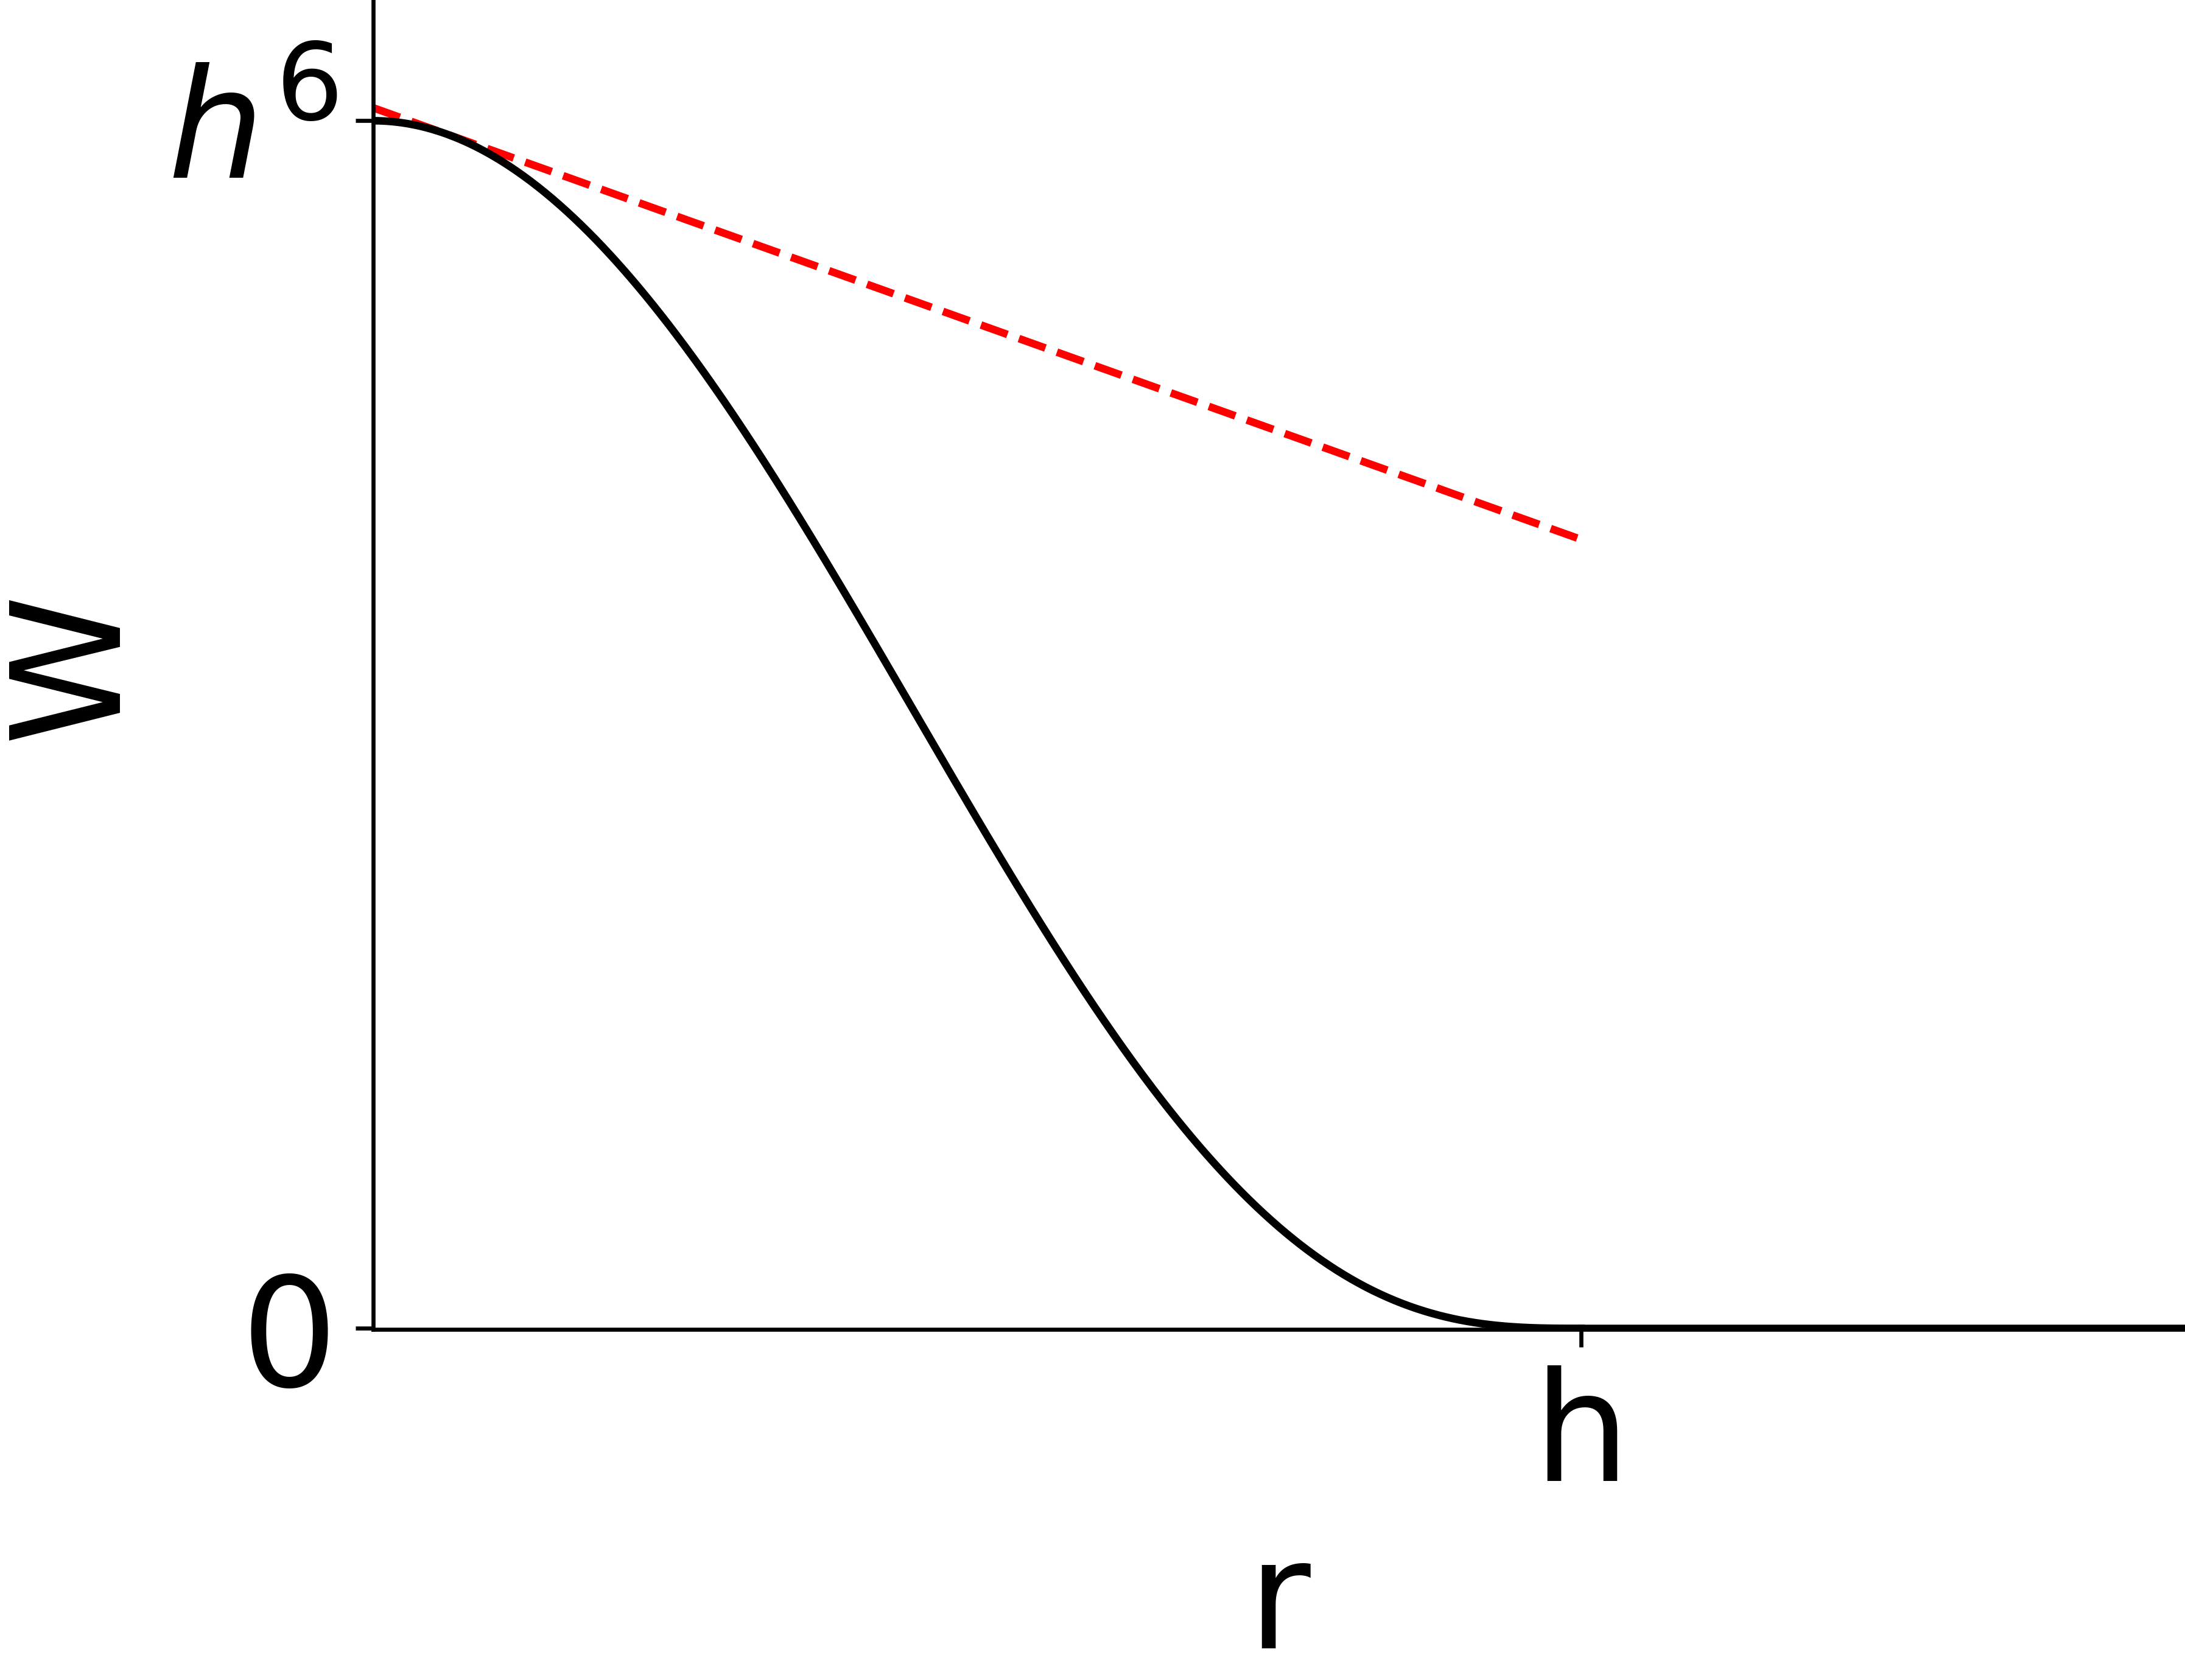
\includegraphics[width=0.9\textwidth]{pictures/slope.png}
\end{figure}
\end{column}
\begin{column}{0.45\textwidth}
\begin{figure}
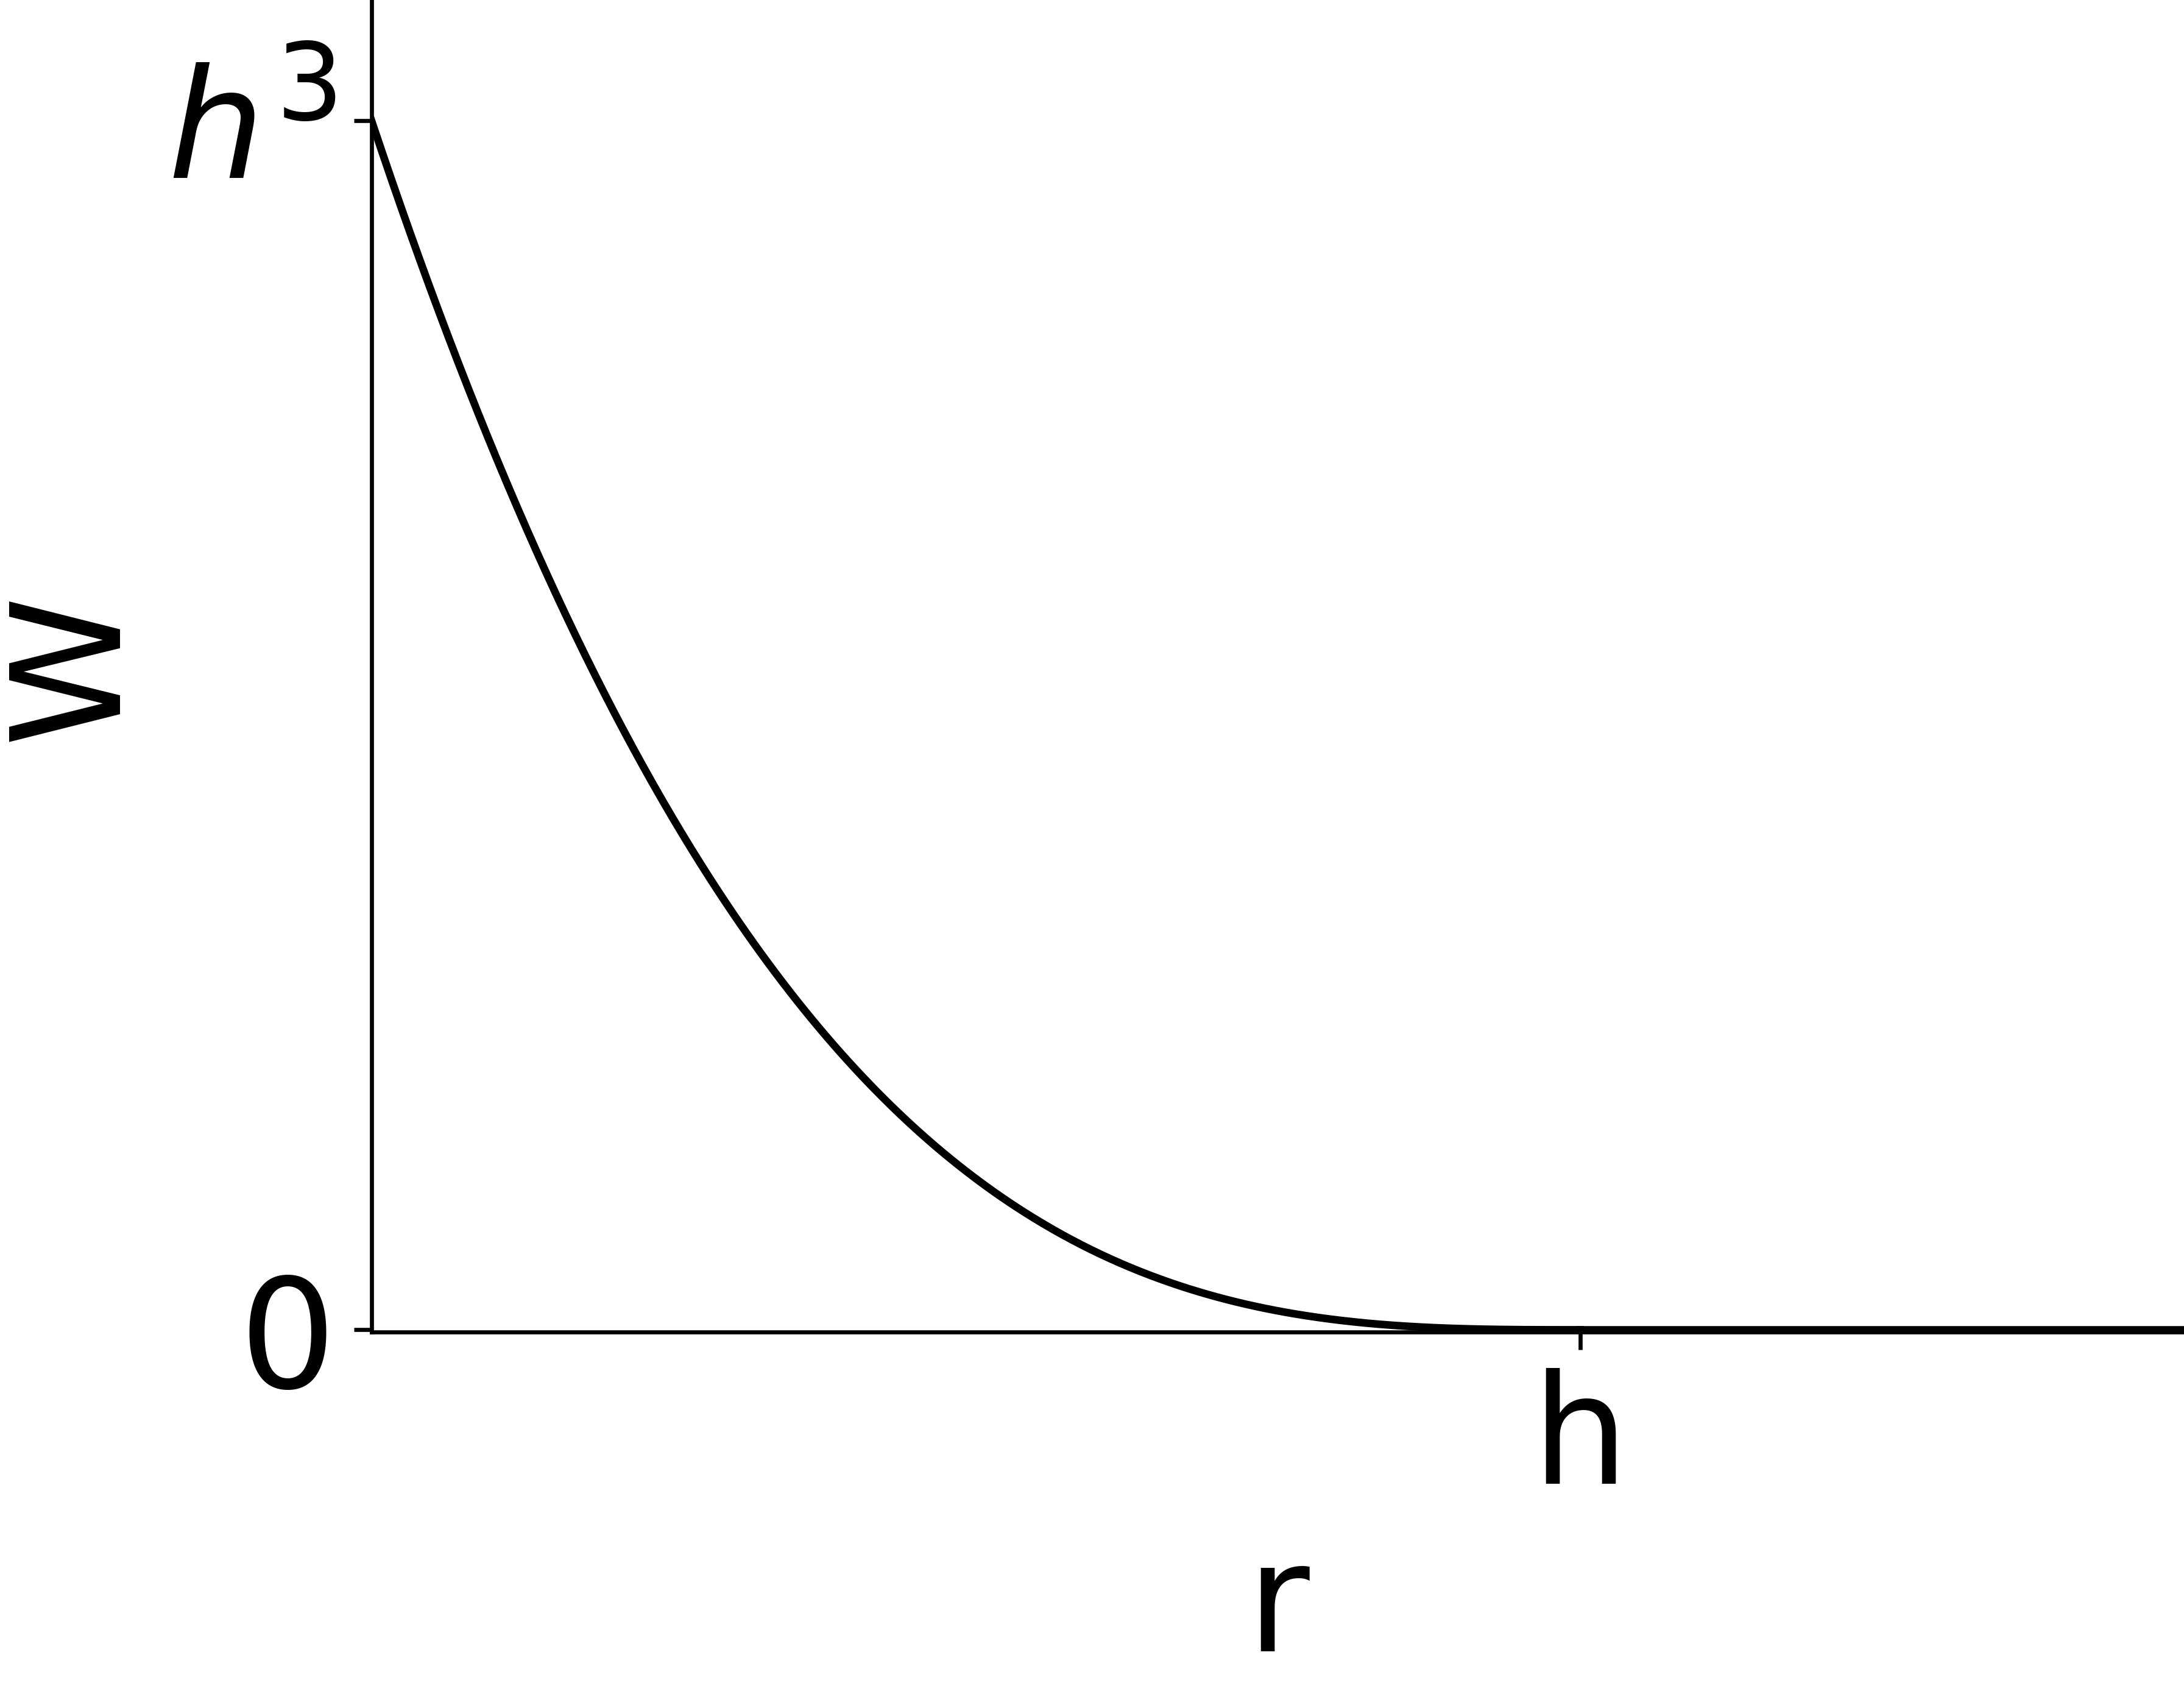
\includegraphics[width=0.9\textwidth]{pictures/smoothing_kernel_2.png}
\end{figure}
\end{column}
\end{columns}
\end{frame}





\begin{frame}
\frametitle{Viscosity}
\begin{columns}
\begin{column}{0.45\textwidth}
\[
W\left(\mathbf{r}, h\right) = 
\begin{cases} 
    \left(h-\left|\mathbf{r}\right|\right)^3 & 0 \leq \left|\mathbf{r}\right| \leq h \\ 
    0 & \text{otherwise.}
\end{cases}
\]
\end{column}
\begin{column}{0.45\textwidth}
{\small\[
W\left(\mathbf{r}, h\right) = 
\begin{cases} 
    -\frac{r^3}{2h^3}+\frac{r^2}{h^2}+\frac{h}{2r}-1 & 0 \leq \left|\mathbf{r}\right| \leq h \\ 
    0 & \text{otherwise.}
\end{cases}
\]}
\end{column}
\end{columns}

\begin{columns}
\begin{column}{0.45\textwidth}
\begin{figure}
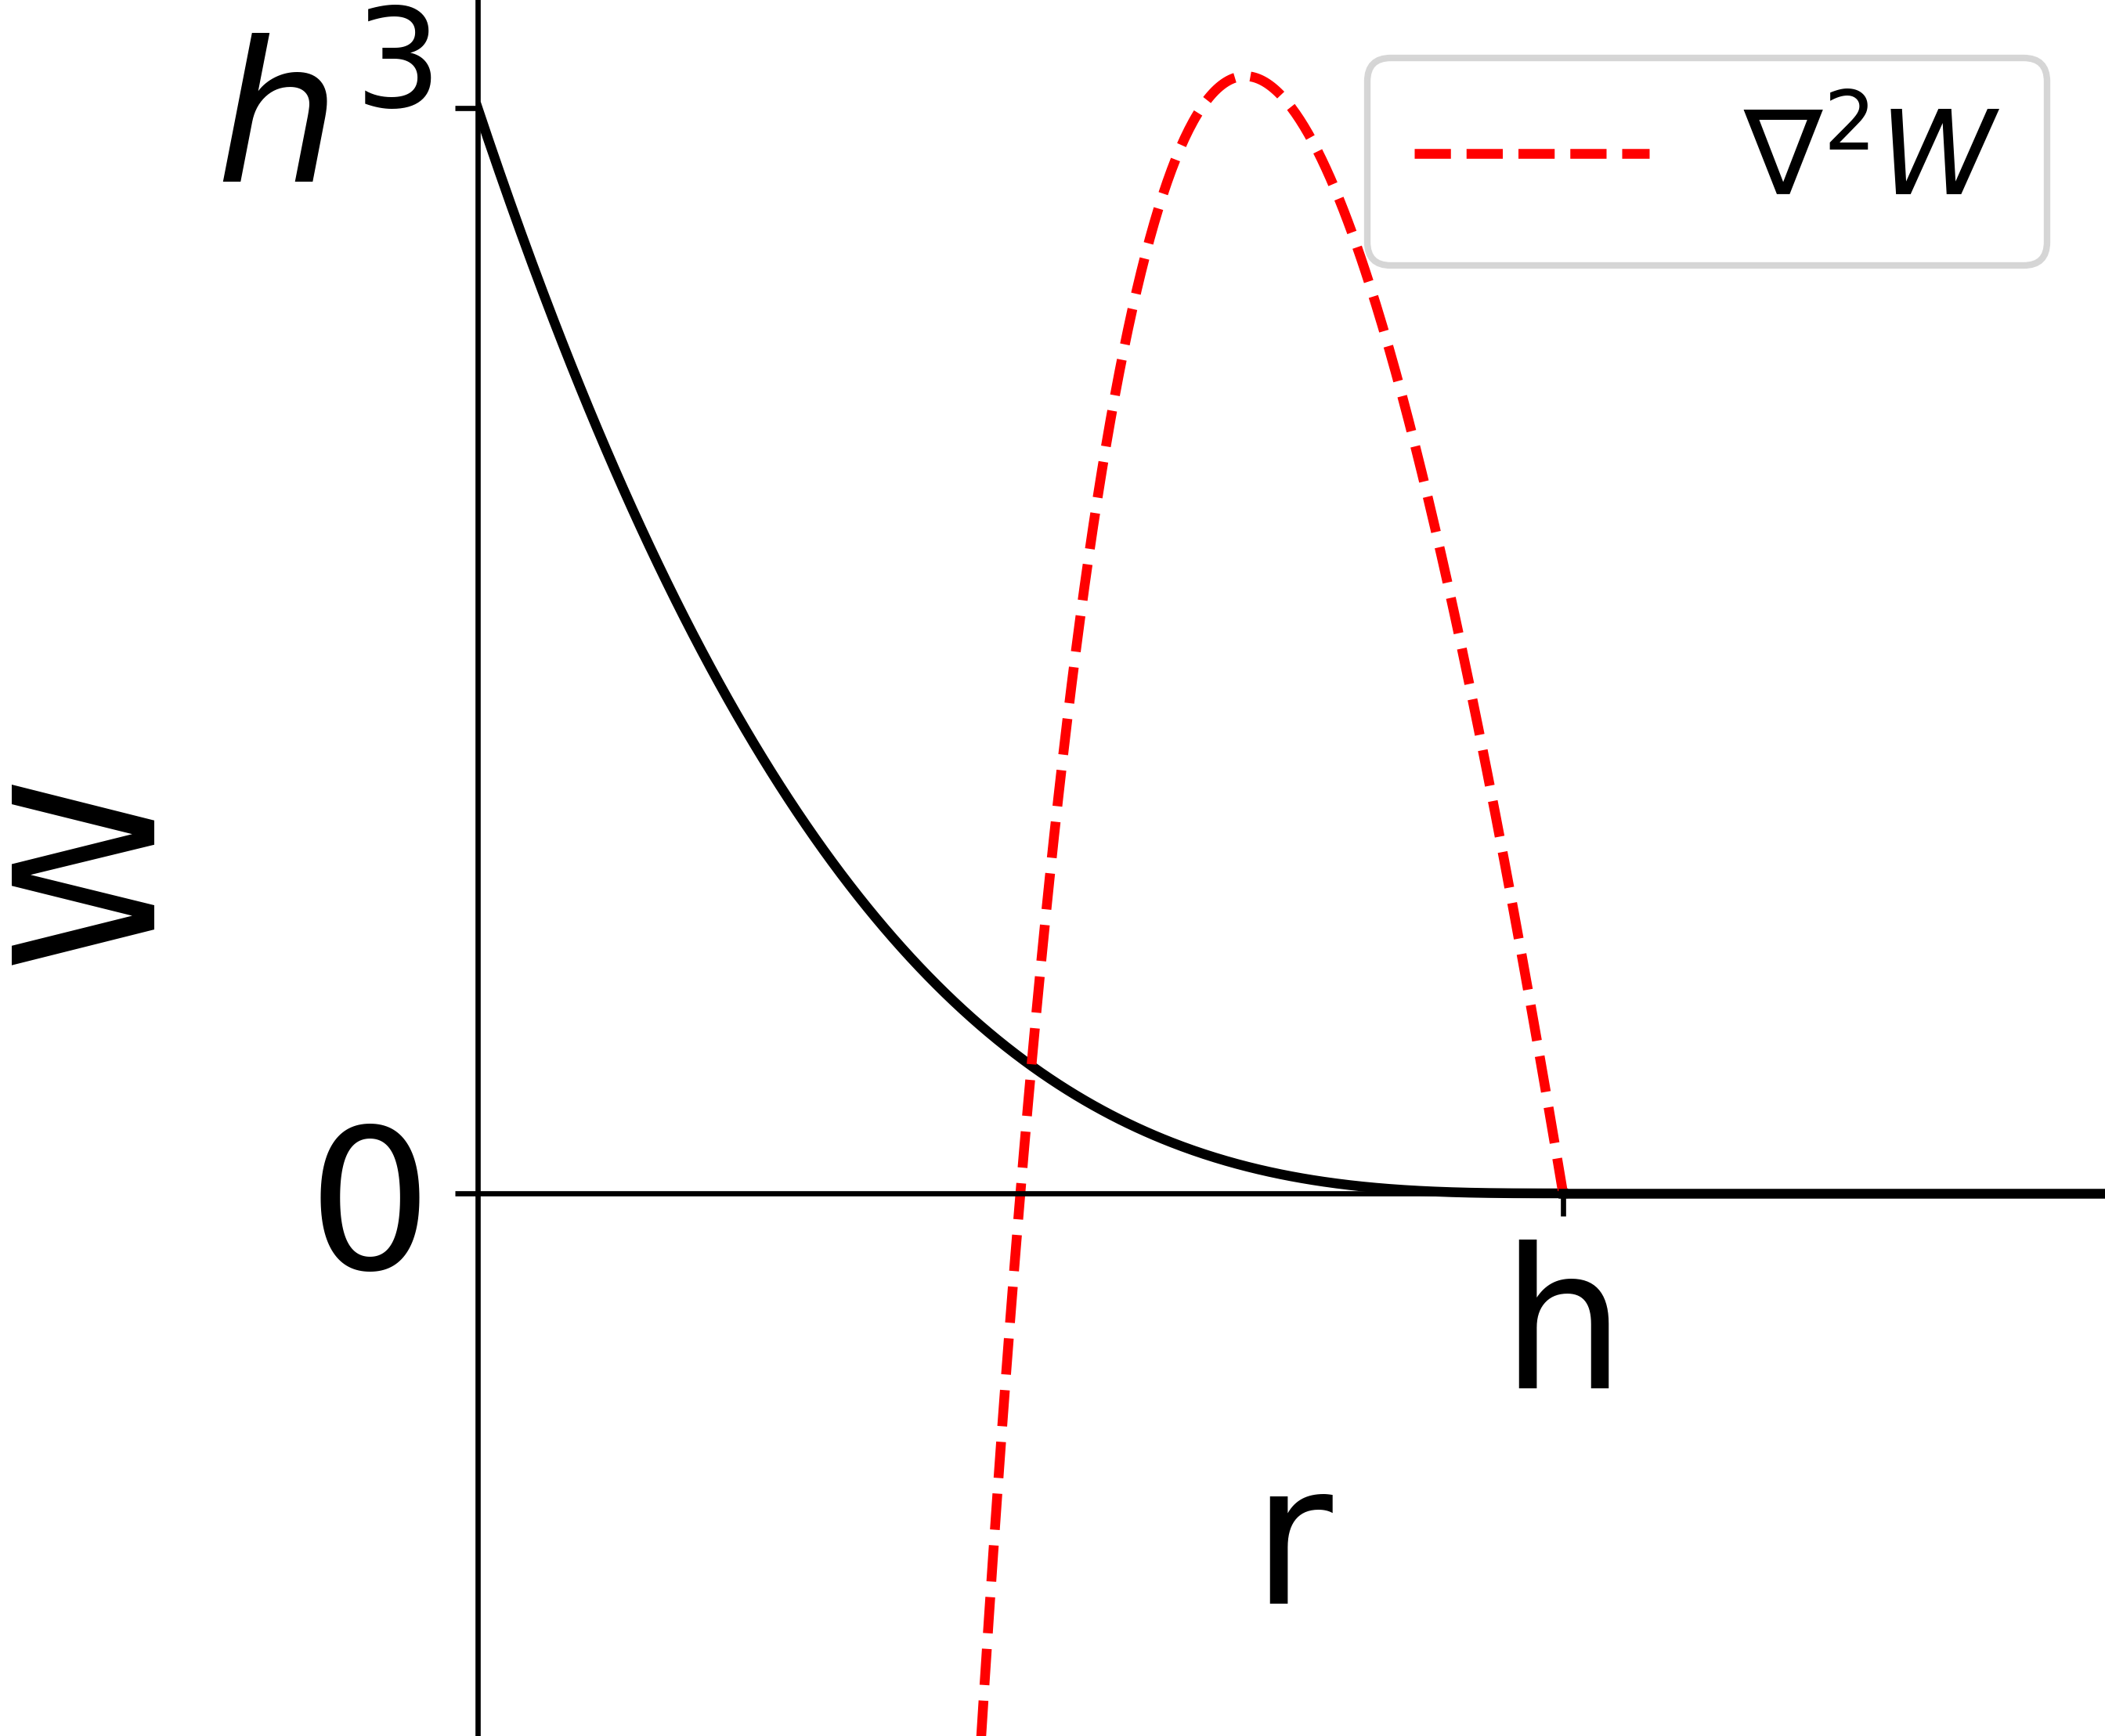
\includegraphics[width=0.9\textwidth]{pictures/laplacian.png}
\end{figure}
\end{column}
\begin{column}{0.45\textwidth}
\begin{figure}
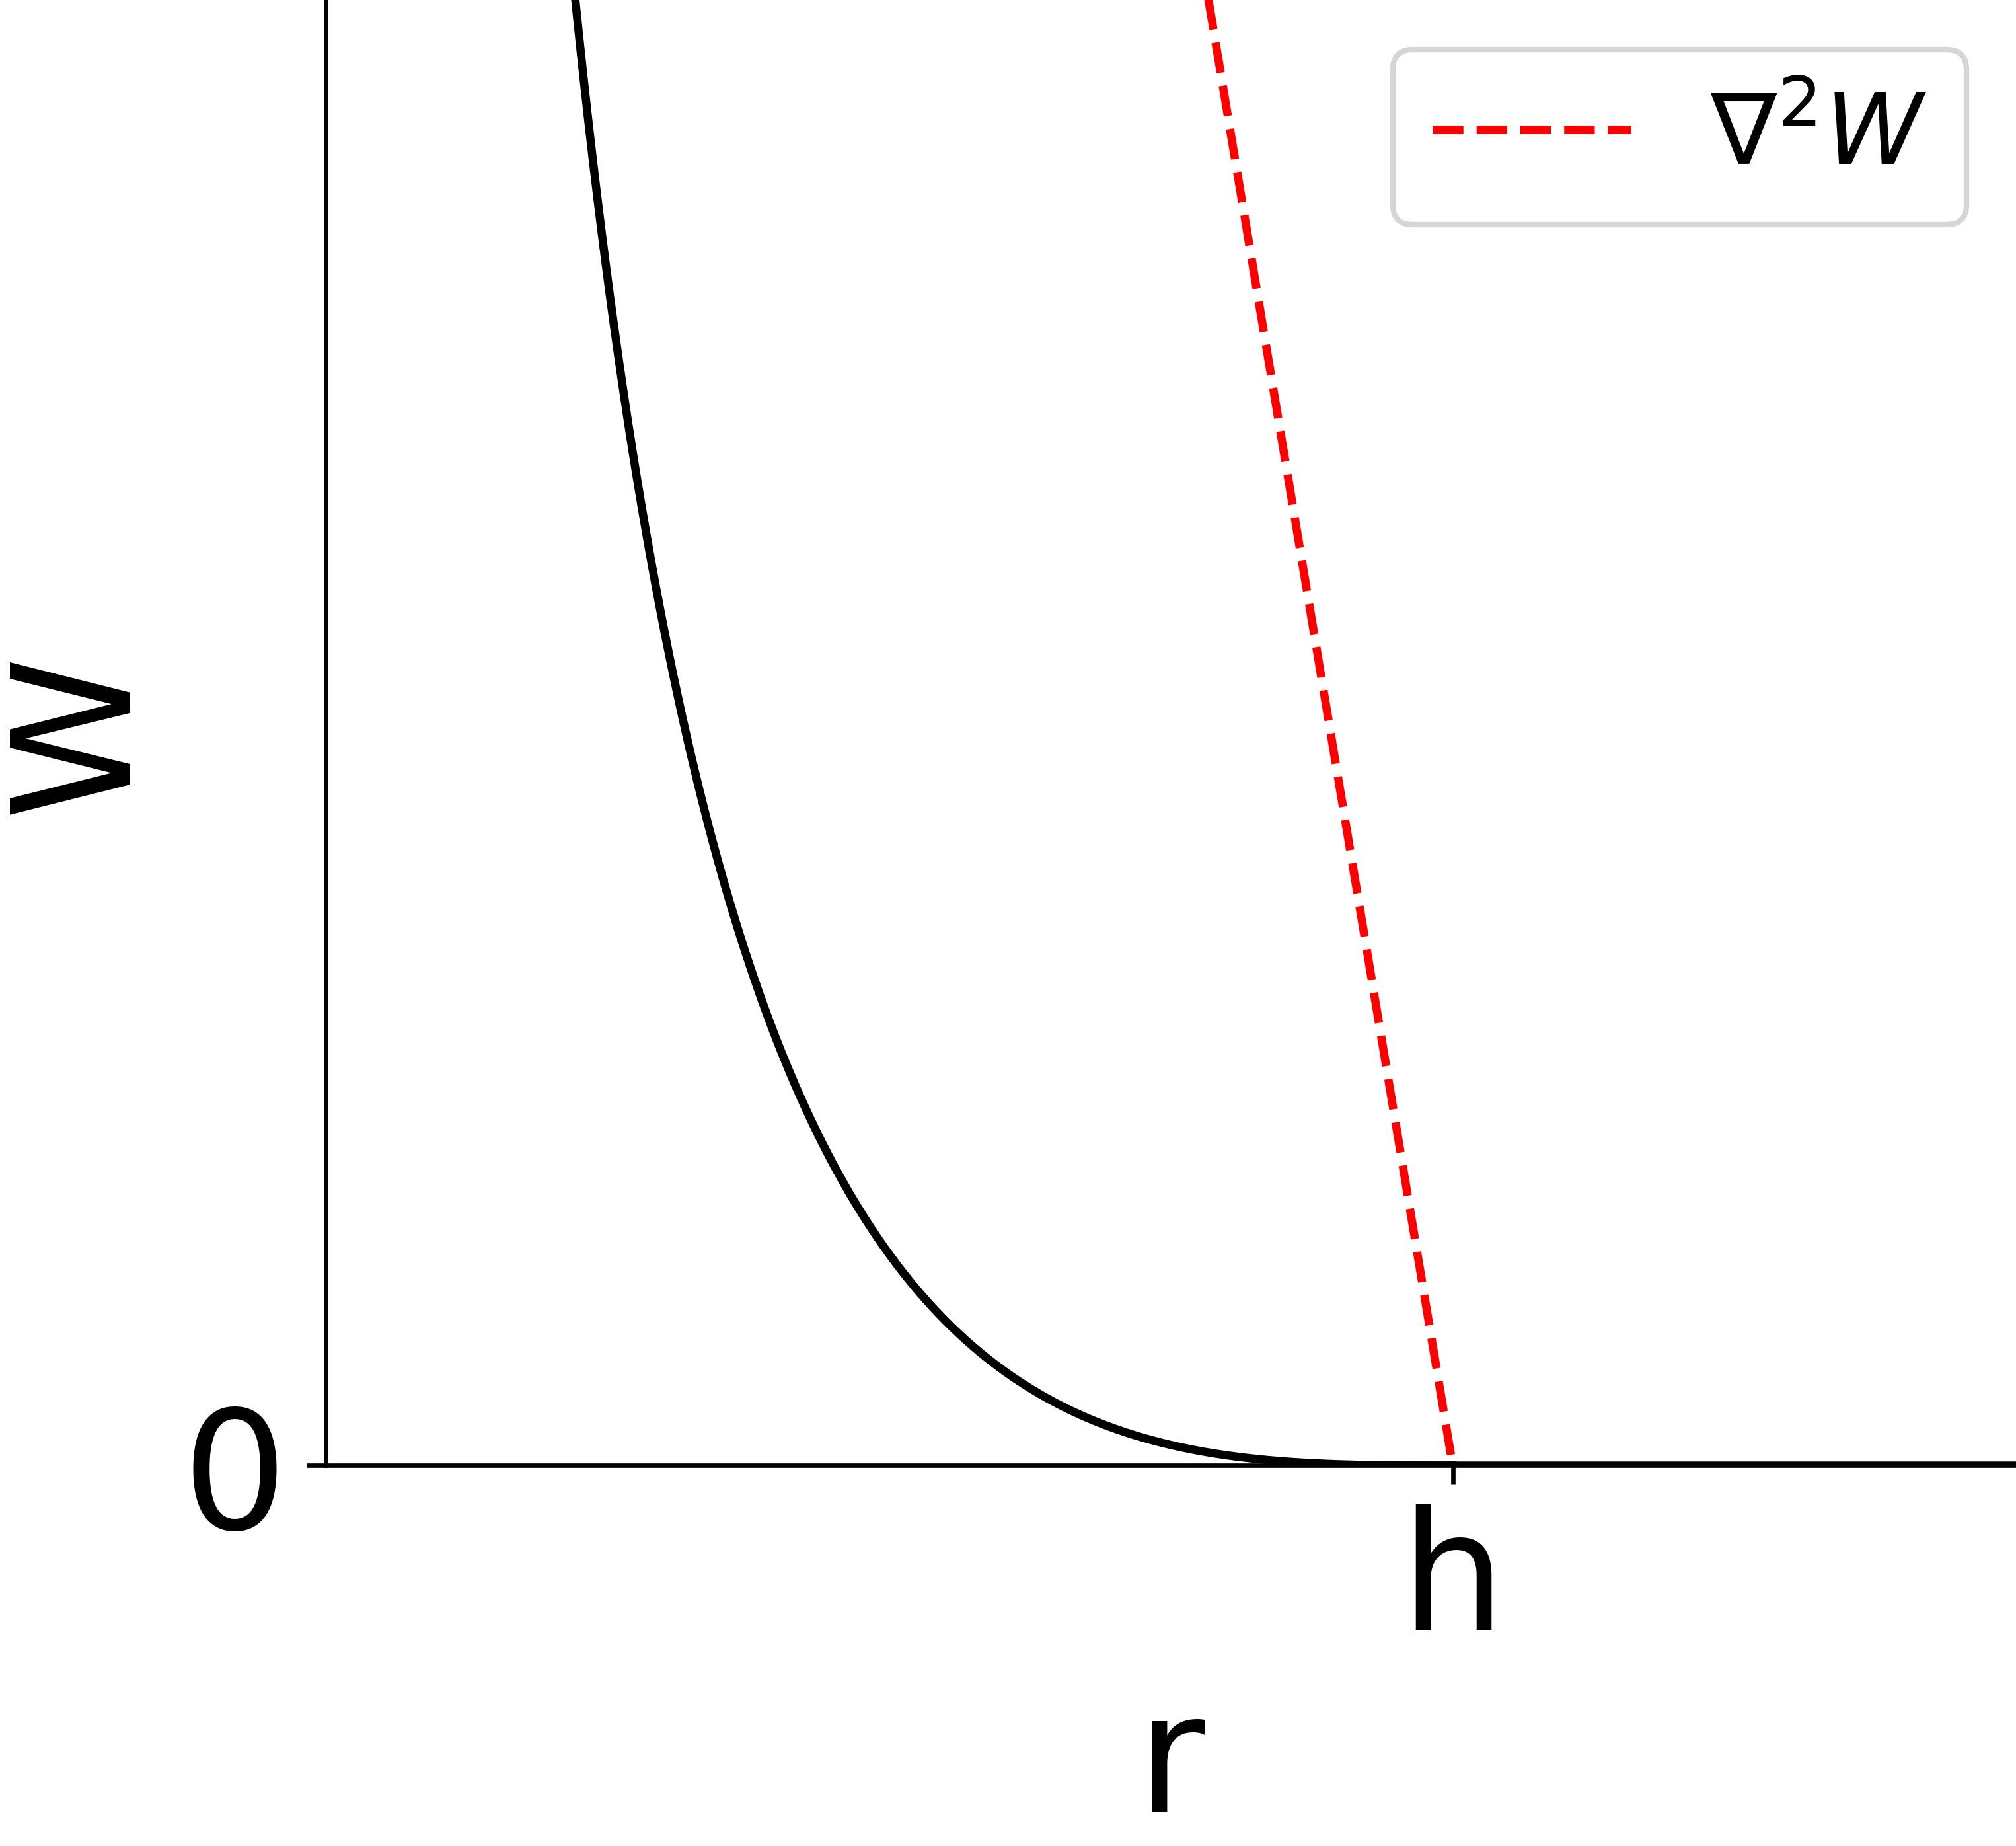
\includegraphics[width=0.9\textwidth]{pictures/laplacian1.png}
\end{figure}
\end{column}
\end{columns}
\end{frame}





\begin{frame}
\frametitle{Normalisation}
\begin{itemize}
\item Slight catch! If you try to change \(h\), \(\rho\) will also change!
\pause
\item Normalisation condition for smoothing kernel:
\end{itemize}
\[
\int W\left(\mathbf{r}, h\right) \text{d}\mathbf{r} = 1.
\]
\pause
\begin{columns}
\begin{column}{0.45\textwidth}
\begin{block}{Density}
\vspace{-1em}
{\small\[
W\left(\mathbf{r}, h\right) = \frac{315}{64\pi h^9}
\begin{cases} 
    \left(h^2-\left|\mathbf{r}\right|^2\right)^3 & 0 \leq \left|\mathbf{r}\right| \leq h \\ 
    0 & \text{otherwise.}
\end{cases}
\]}
\end{block}
\end{column}


\begin{column}{0.45\textwidth}
\begin{block}{Pressure}
\vspace{-1em}
{\small\[
W\left(\mathbf{r}, h\right) = \frac{15}{\pi h^6}
\begin{cases} 
    \left(h-\left|\mathbf{r}\right|\right)^3 & 0 \leq \left|\mathbf{r}\right| \leq h \\ 
    0 & \text{otherwise.}
\end{cases}
\]}
\end{block}
\end{column}
\end{columns}


\begin{columns}
\begin{column}{0.18\textwidth}
\end{column}
\begin{column}{0.54\textwidth}
\begin{block}{Viscosity}
\vspace{-1em}
{\small\[
W\left(\mathbf{r}, h\right) = \frac{15}{2\pi h^3}
\begin{cases} 
    -\frac{r^3}{2h^3}+\frac{r^2}{h^2}+\frac{h}{2r}-1 & 0 \leq \left|\mathbf{r}\right| \leq h \\ 
    0 & \text{otherwise.}
\end{cases}
\]}
\end{block}
\end{column}
\begin{column}{0.18\textwidth}
\end{column}
\end{columns}
\end{frame}





\begin{frame}
\frametitle{Grid Data Structure}
\begin{itemize}
\item Do we really need to loop over all particles when we use interpolating equation?
\end{itemize}
\begin{figure}
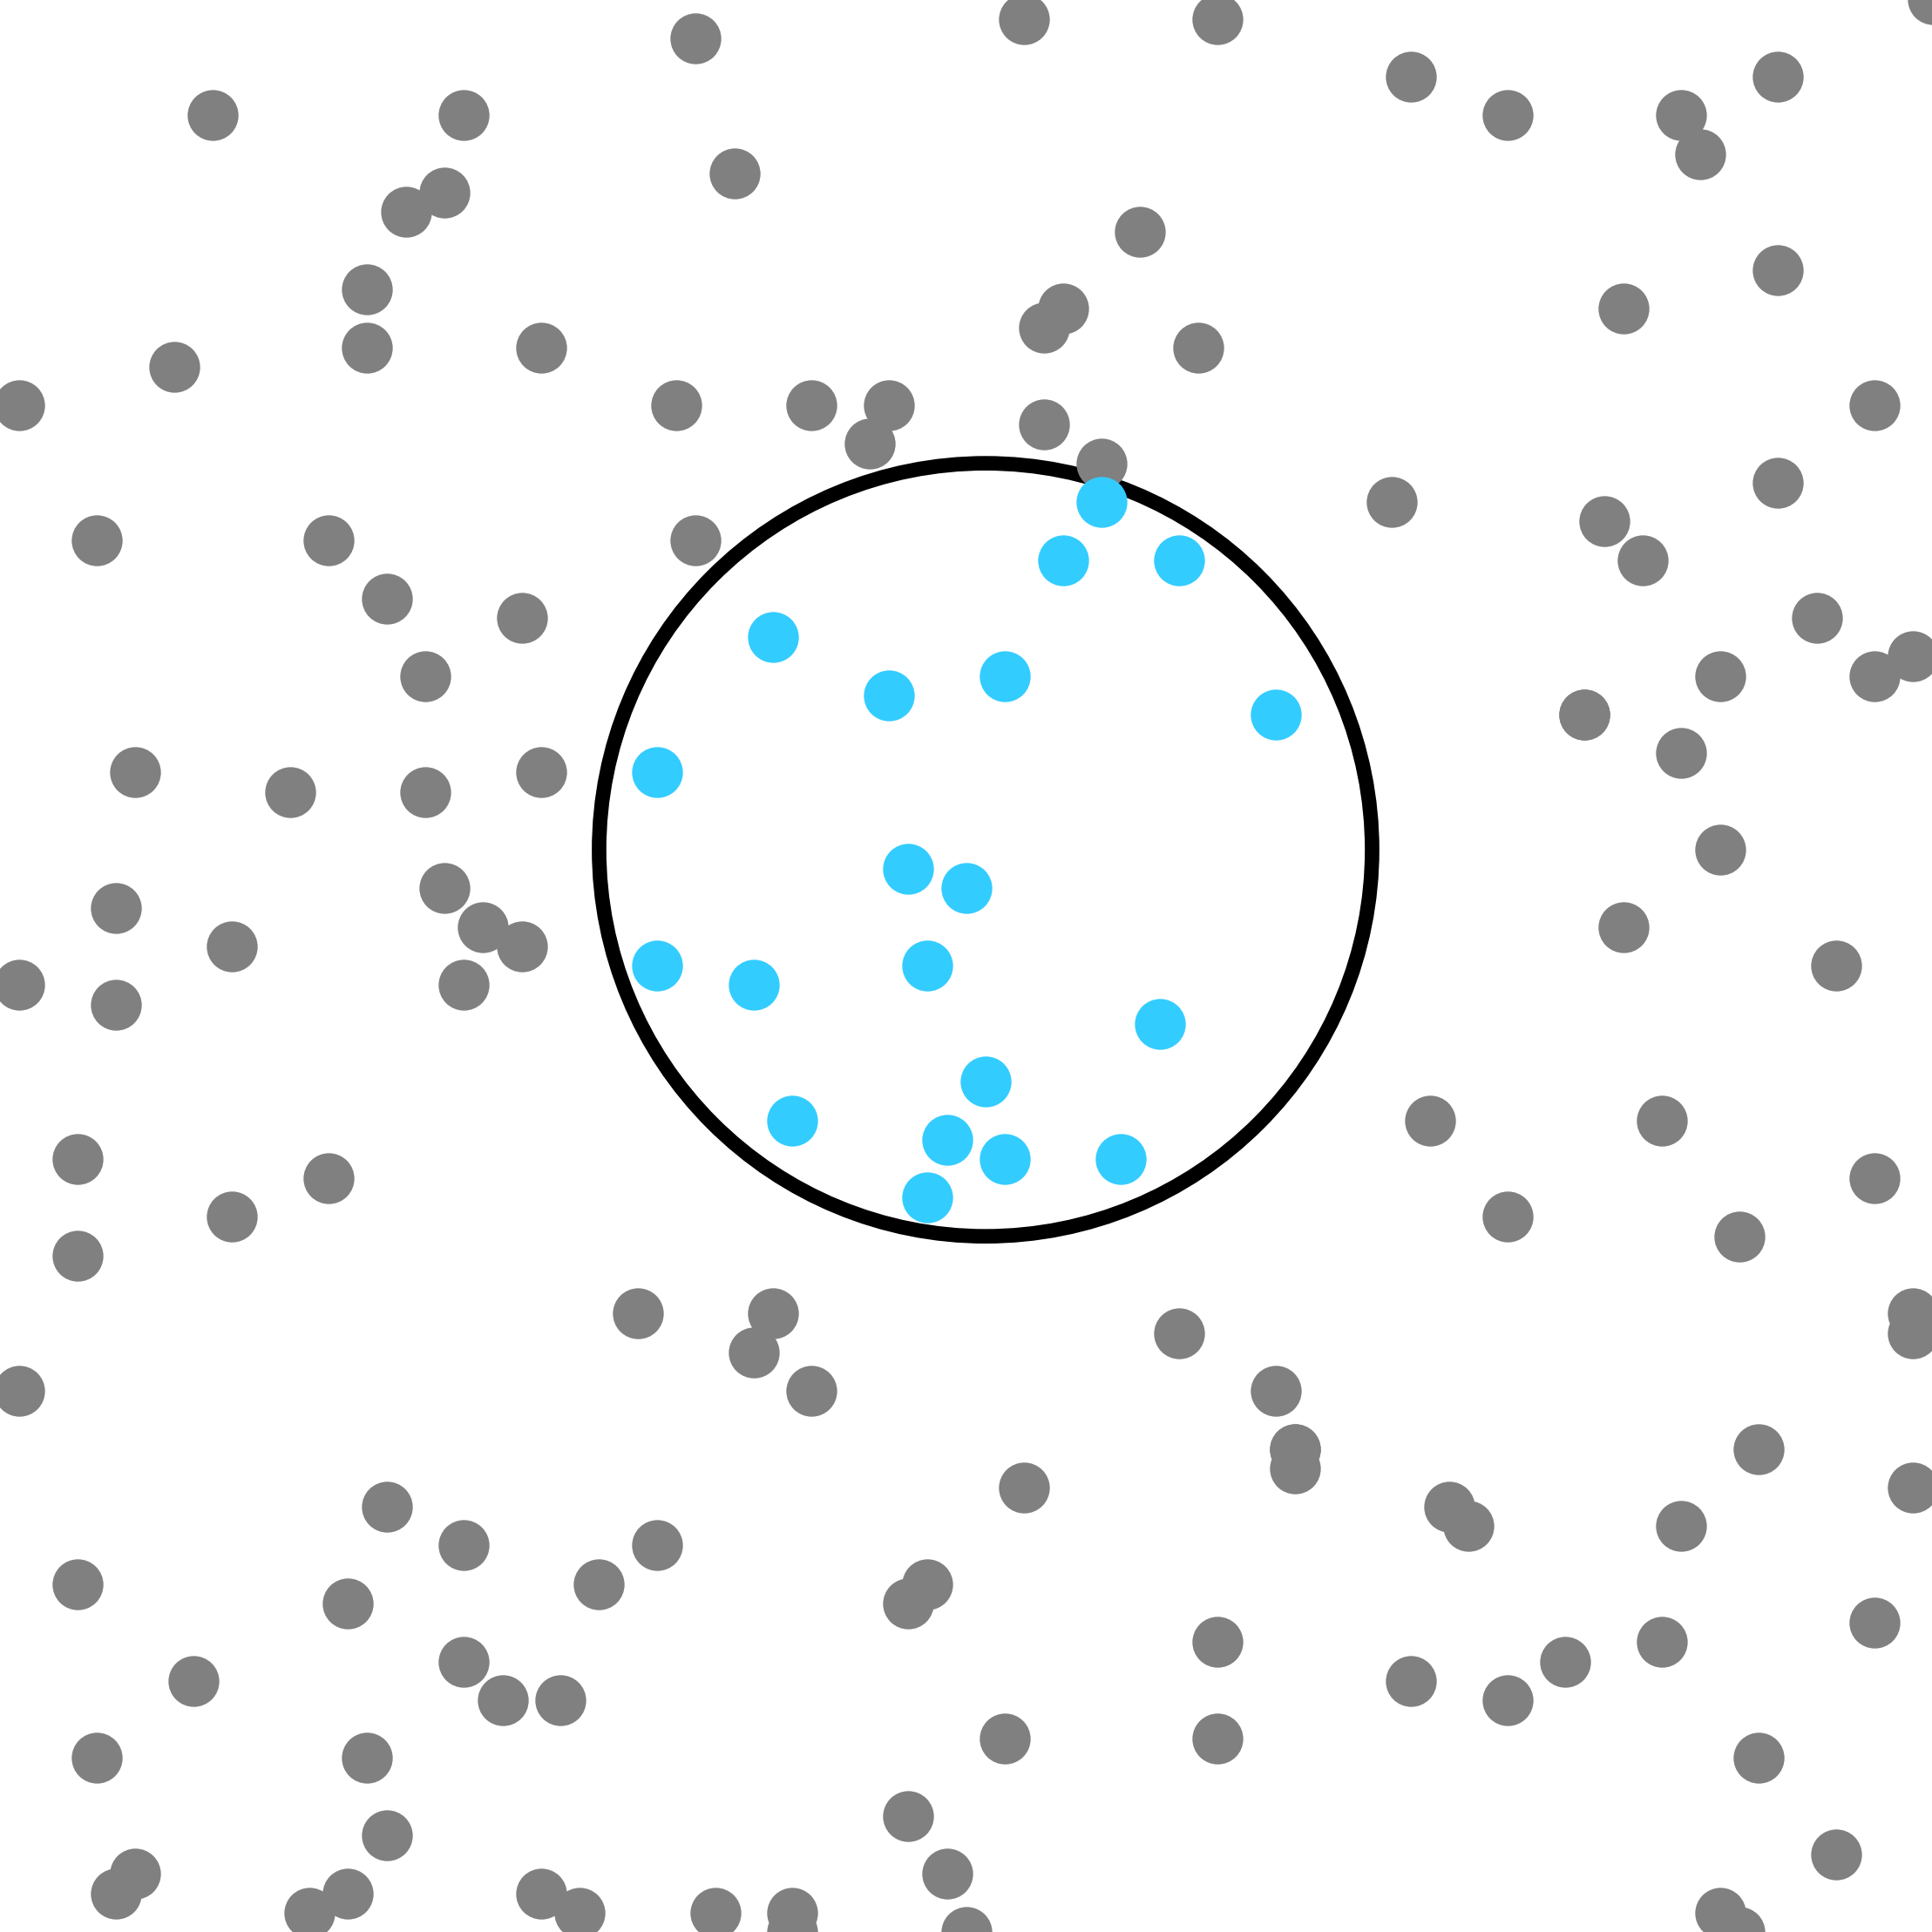
\includegraphics[width=0.4\textwidth]{pictures/grid1.png}
\end{figure}
\end{frame}





\begin{frame}
\frametitle{Grid Data Structure}
\begin{itemize}
\item Do we really need to loop over all particles when we use interpolating equation?
\end{itemize}
\begin{figure}
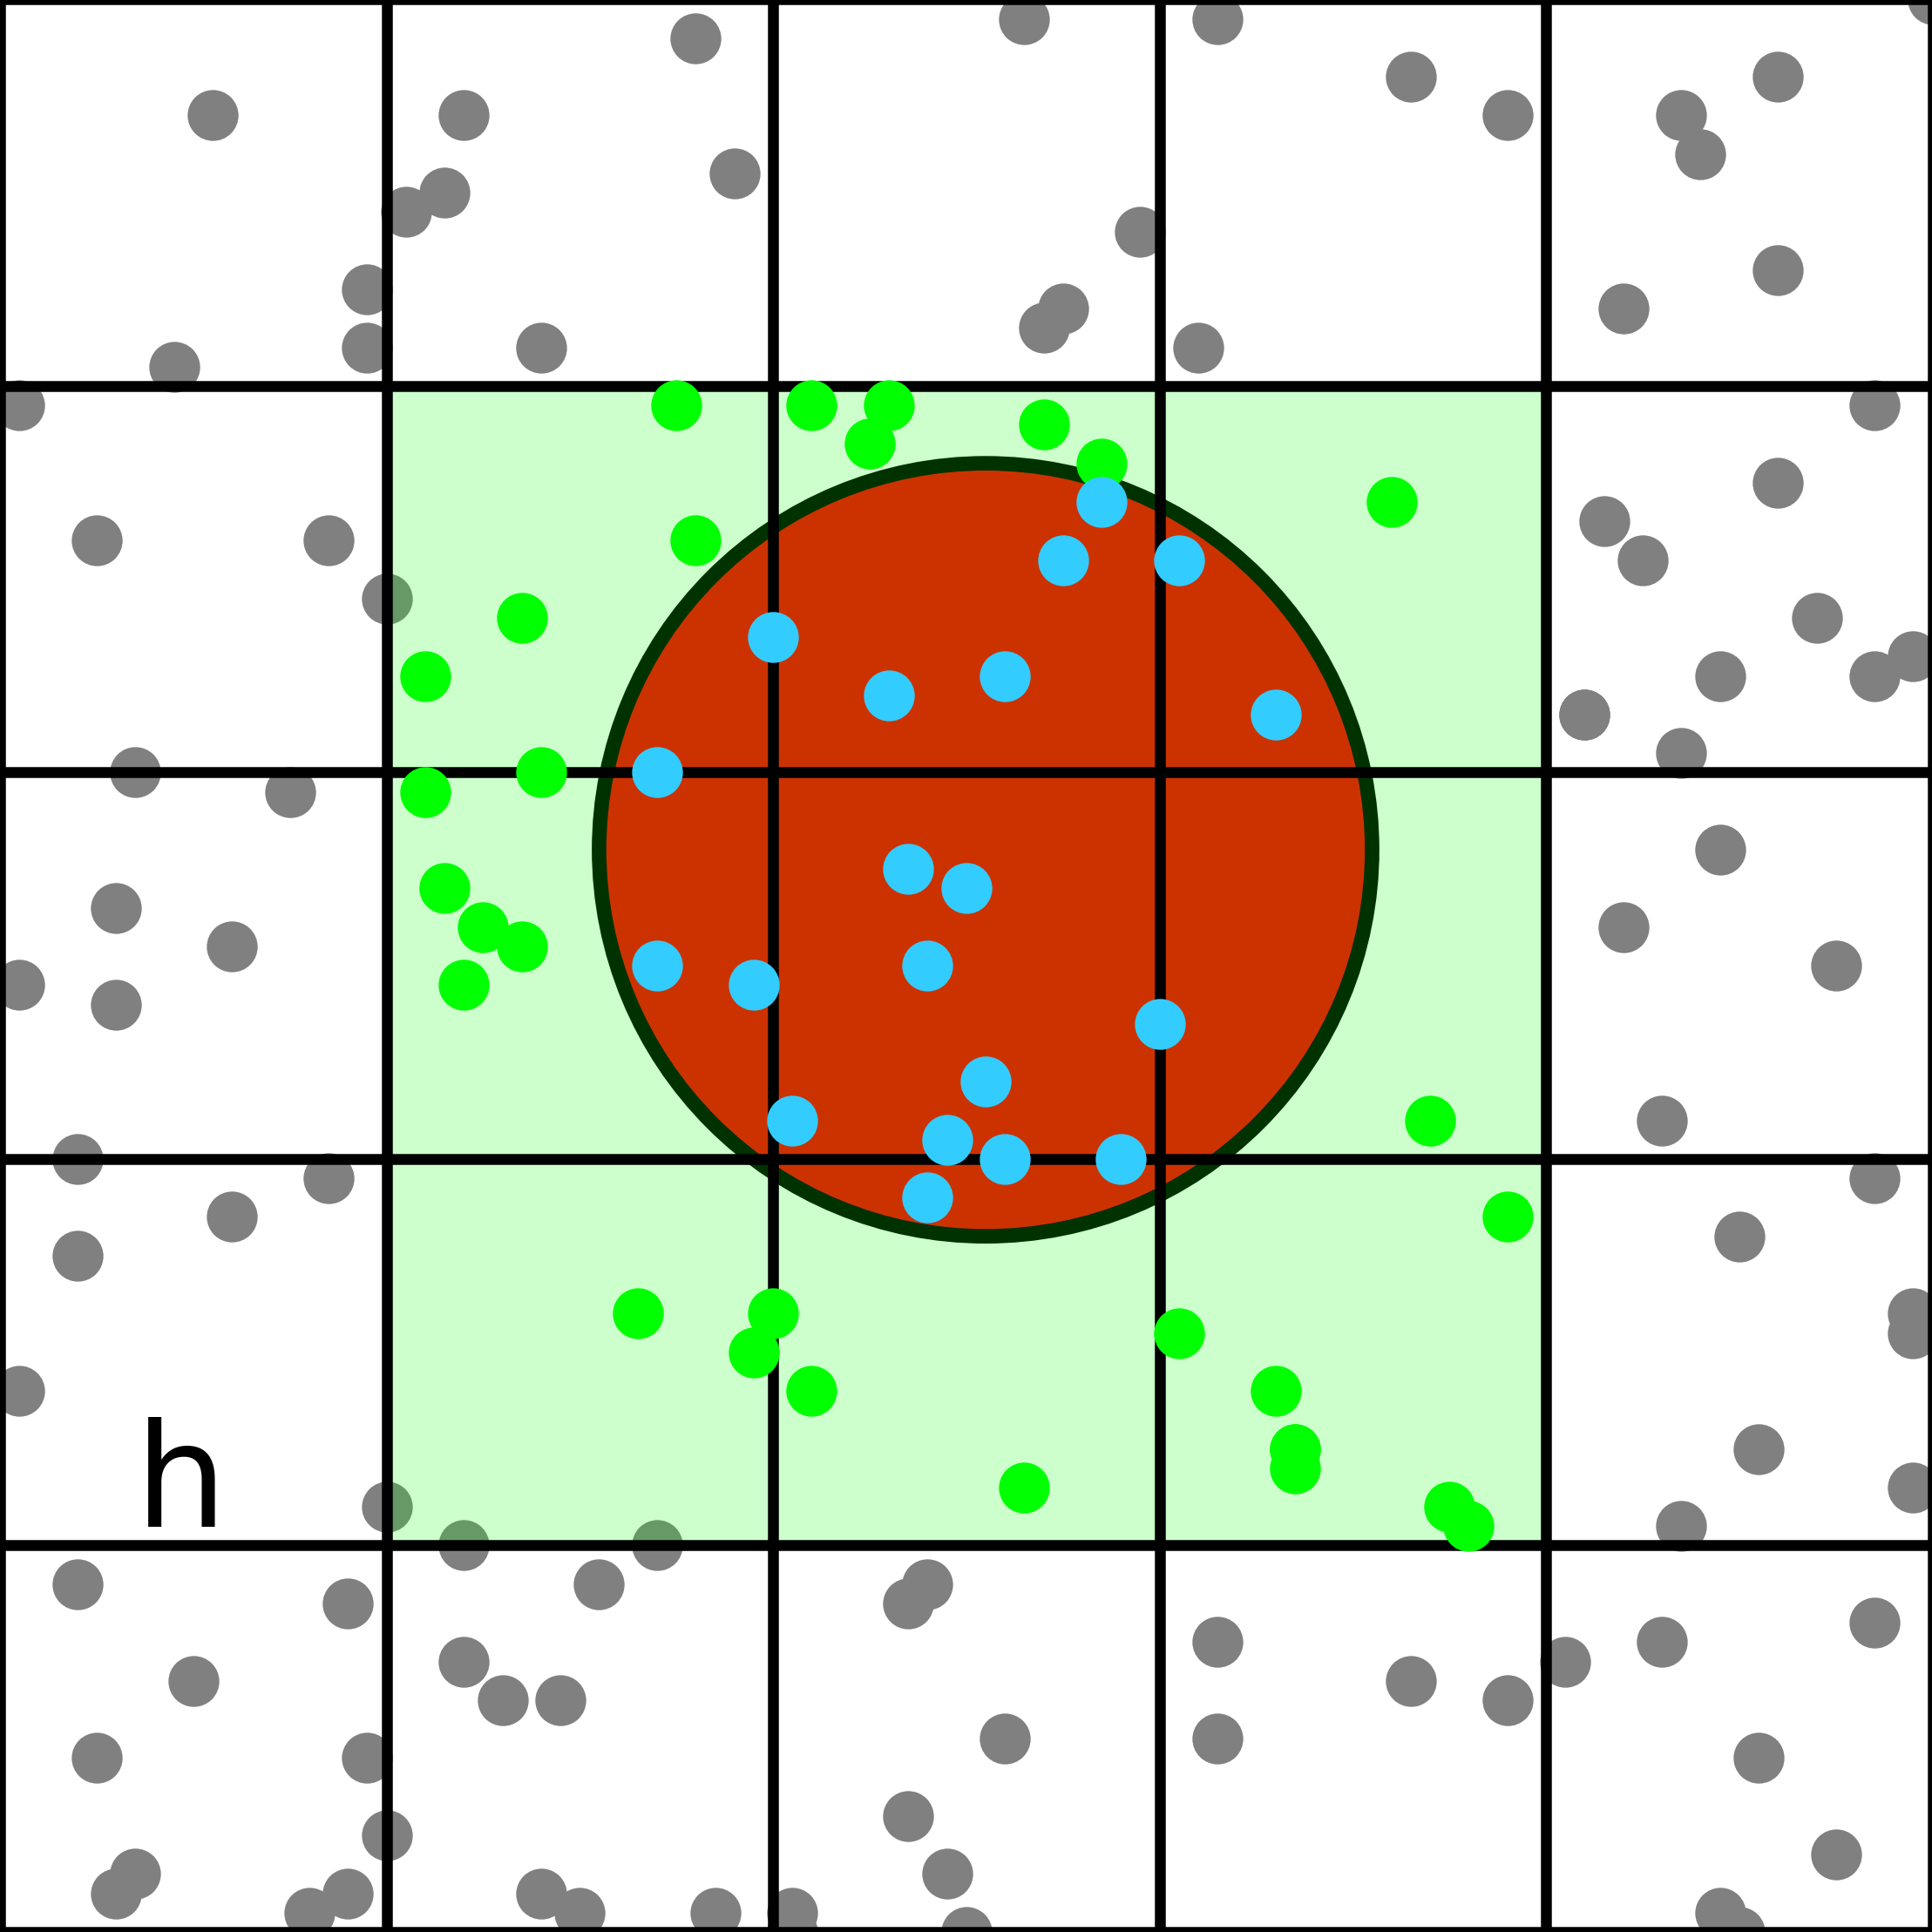
\includegraphics[width=0.4\textwidth]{pictures/grid2.png}
\end{figure}
\end{frame}





\begin{frame}
\frametitle{Grid Data Structure}
\begin{align*}
\texttt{\textcolor{blue}{int} particle\_index[\textcolor{purple}{10}]} &\texttt{ = \{\textcolor{purple}{0}, \textcolor{purple}{1}, \textcolor{purple}{2}, \textcolor{purple}{3}, \textcolor{purple}{4}, \textcolor{purple}{5}, \textcolor{purple}{6}, \textcolor{purple}{7}, \textcolor{purple}{8}, \textcolor{purple}{9}\};} \\
\texttt{\textcolor{blue}{int} cell\_id[\textcolor{purple}{10}]} &\texttt{ = \{\textcolor{purple}{5}, \textcolor{purple}{7}, \textcolor{purple}{5}, \textcolor{purple}{8}, \textcolor{purple}{0}, \textcolor{purple}{8}, \textcolor{purple}{7}, \textcolor{purple}{5}, \textcolor{purple}{5}, \textcolor{purple}{8}\};}
\end{align*}
\begin{figure}
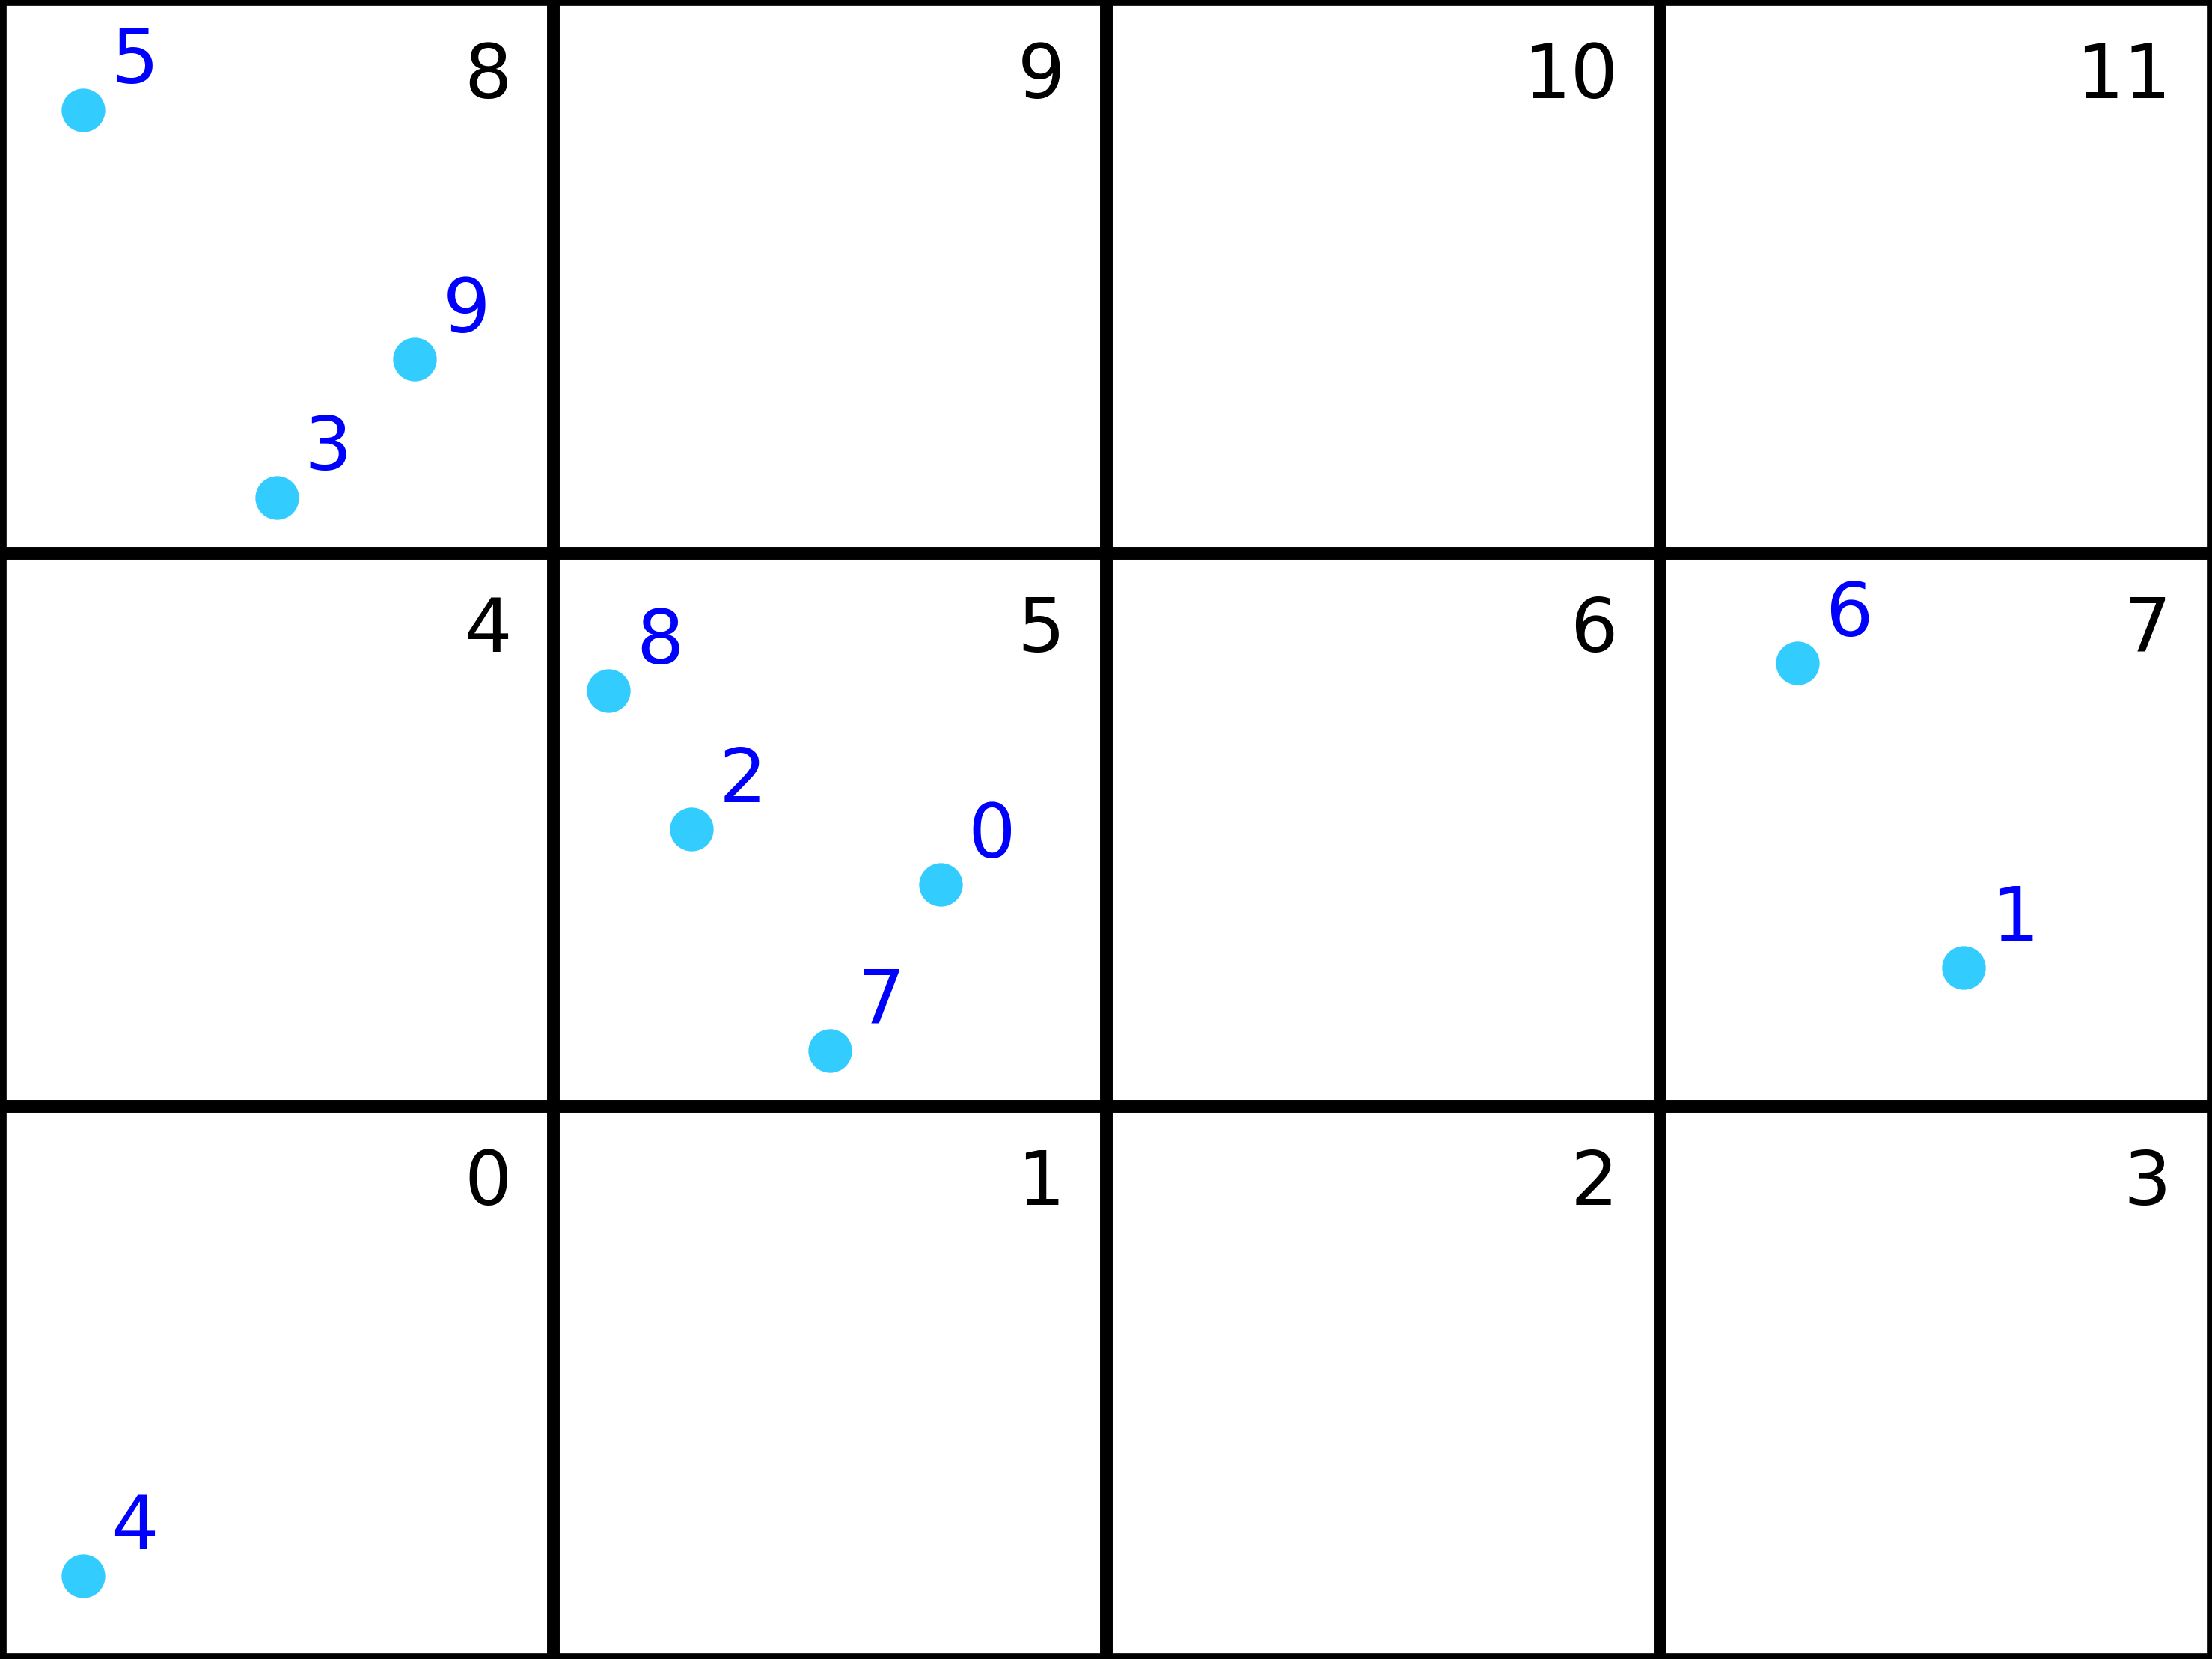
\includegraphics[width=0.4\textwidth]{pictures/grid3.png}
\end{figure}
\end{frame}





\begin{frame}
\frametitle{Grid Data Structure}
\begin{align*}
\texttt{\textcolor{blue}{int} particle\_index[\textcolor{purple}{10}]} &\texttt{ = \{\textcolor{purple}{4}, \textcolor{purple}{0}, \textcolor{purple}{2}, \textcolor{purple}{7}, \textcolor{purple}{8}, \textcolor{purple}{1}, \textcolor{purple}{6}, \textcolor{purple}{3}, \textcolor{purple}{5}, \textcolor{purple}{9}\};} \\
\texttt{\textcolor{blue}{int} cell\_id[\textcolor{purple}{10}]} &\texttt{ = \{\textcolor{purple}{0}, \textcolor{purple}{5}, \textcolor{purple}{5}, \textcolor{purple}{5}, \textcolor{purple}{5}, \textcolor{purple}{7}, \textcolor{purple}{7}, \textcolor{purple}{8}, \textcolor{purple}{8}, \textcolor{purple}{8}\};}
\end{align*}
\begin{figure}
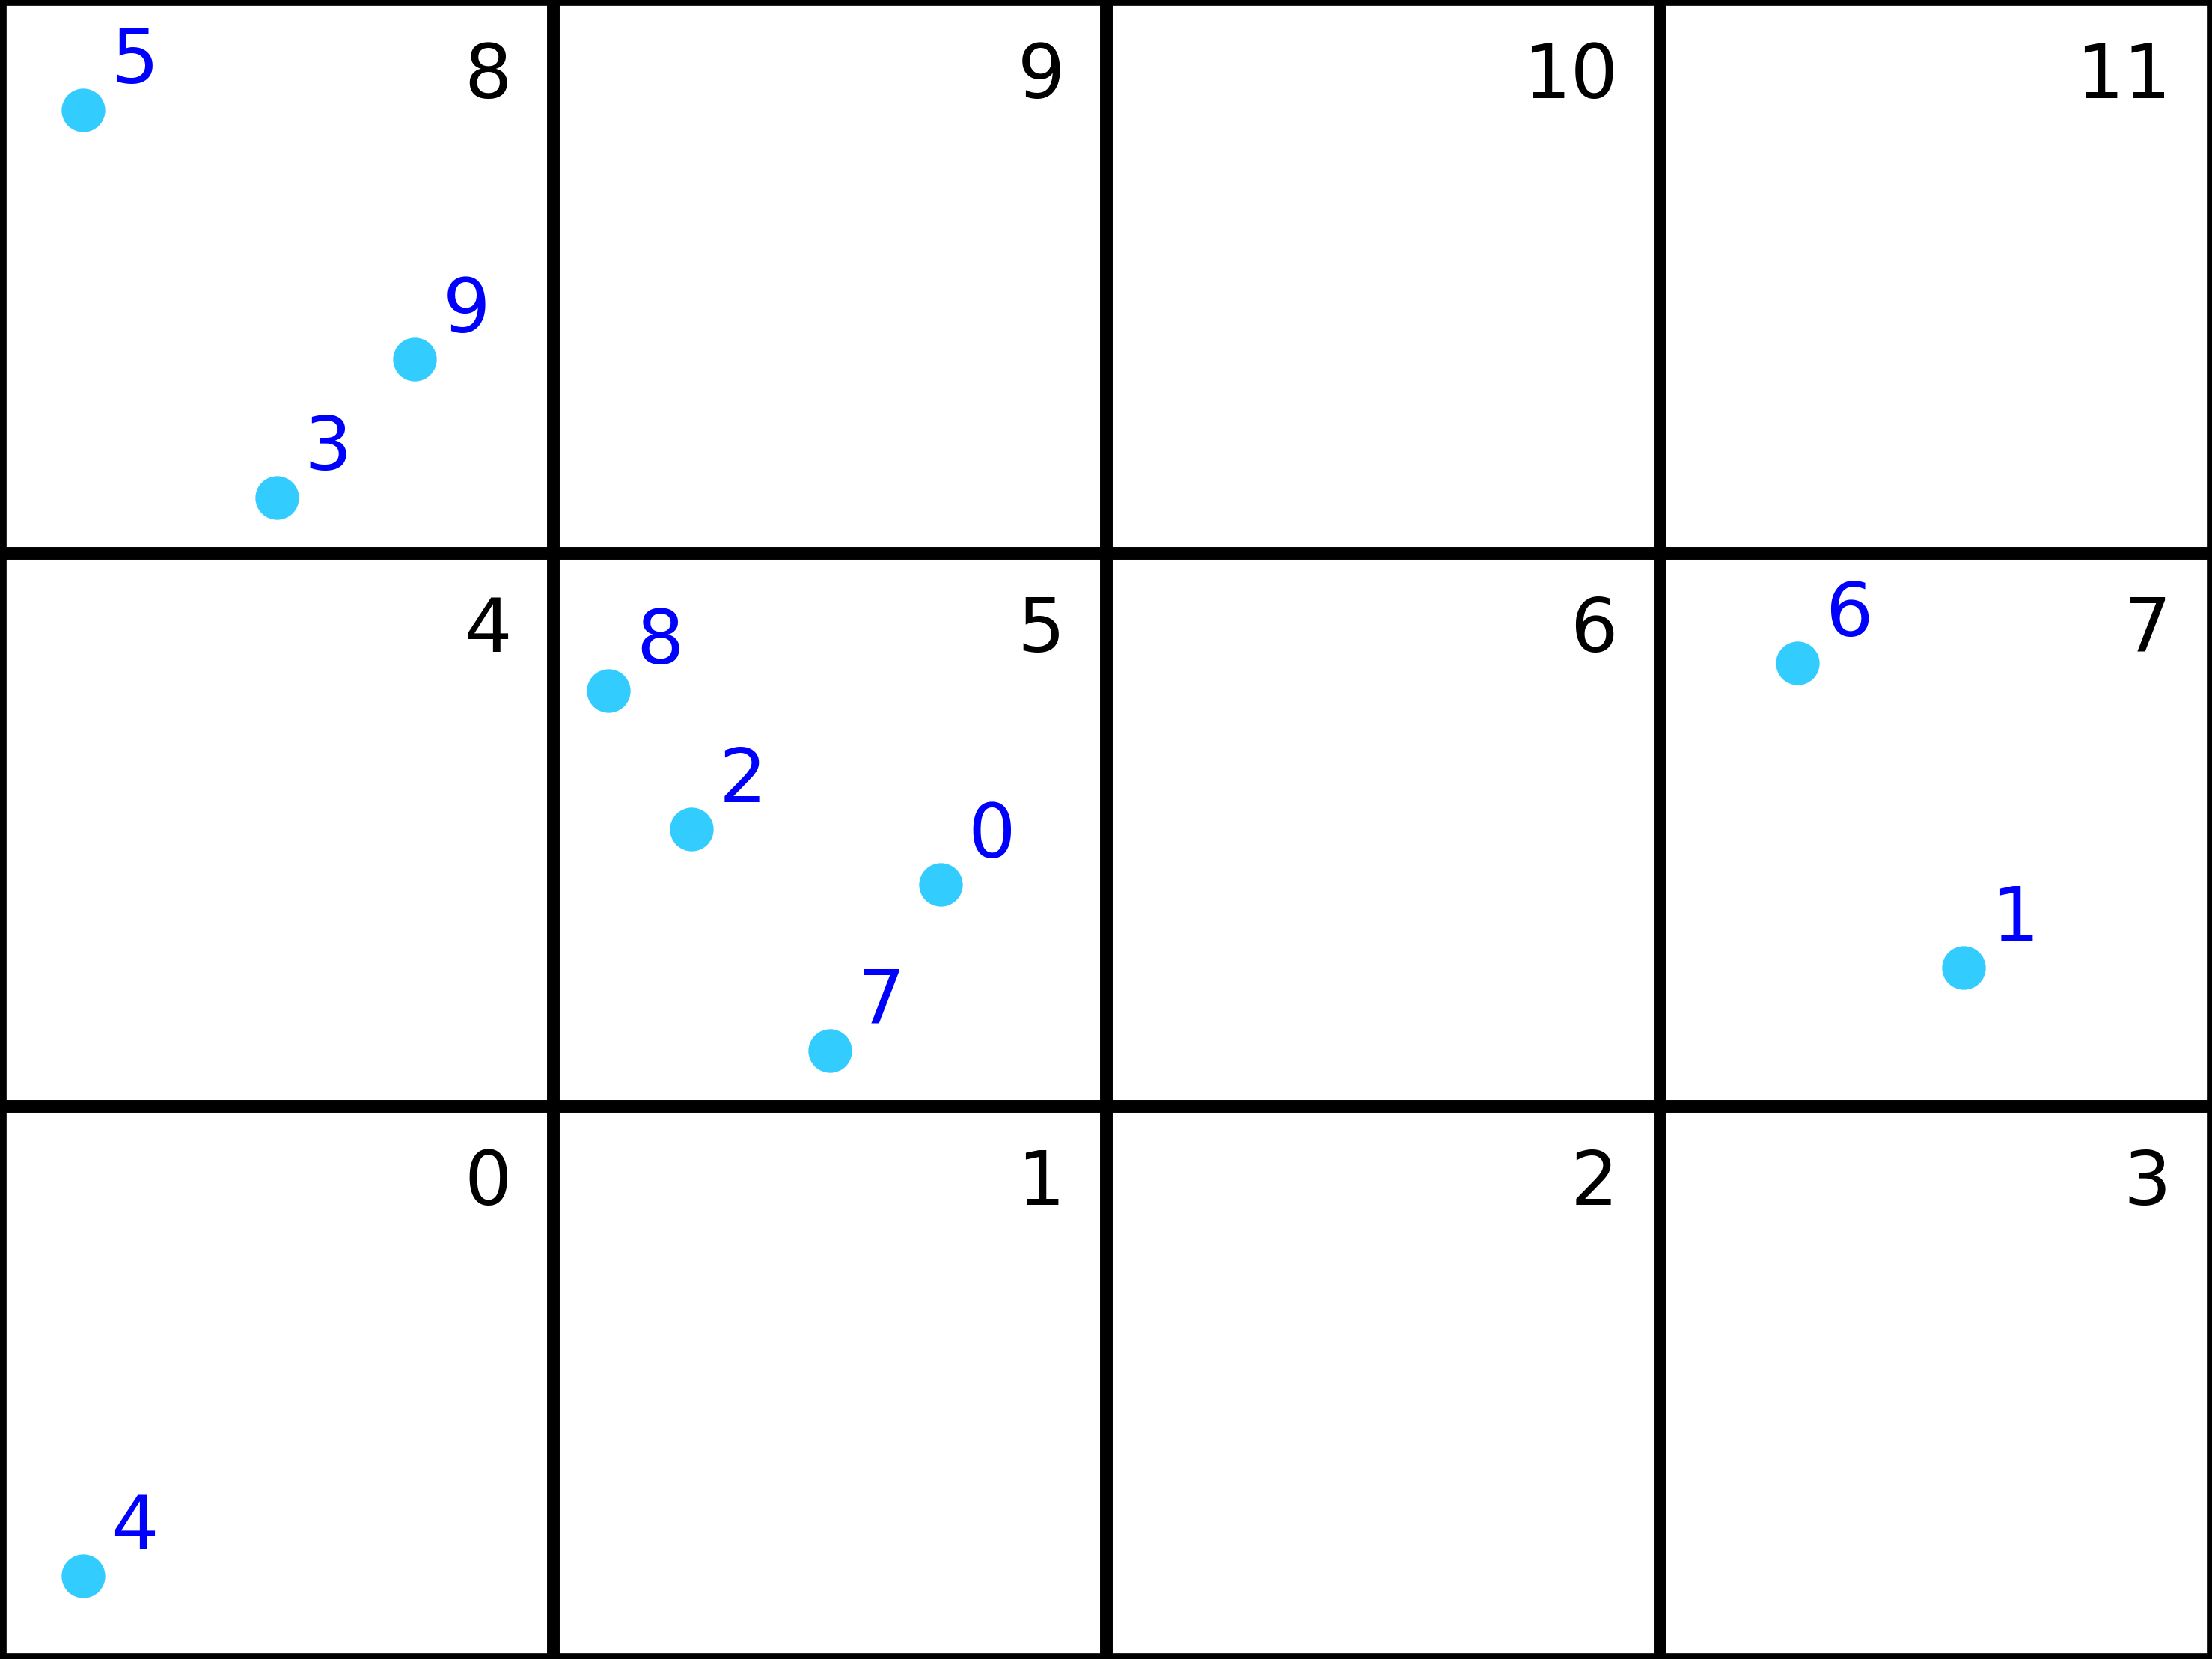
\includegraphics[width=0.4\textwidth]{pictures/grid3.png}
\end{figure}
\end{frame}





\begin{frame}
\frametitle{Grid Data Structure}
\vspace{-1.5em}
\begin{align*}
\texttt{\textcolor{blue}{int} particle\_index[\textcolor{purple}{10}]} &\texttt{ = \{\textcolor{purple}{4}, \textcolor{purple}{0}, \textcolor{purple}{2}, \textcolor{purple}{7}, \textcolor{purple}{8}, \textcolor{purple}{1}, \textcolor{purple}{6}, \textcolor{purple}{3}, \textcolor{purple}{5}, \textcolor{purple}{9}\};} \\
\texttt{\textcolor{blue}{int} cell\_id[\textcolor{purple}{10}]} &\texttt{ = \{\textcolor{purple}{0}, \textcolor{purple}{5}, \textcolor{purple}{5}, \textcolor{purple}{5}, \textcolor{purple}{5}, \textcolor{purple}{7}, \textcolor{purple}{7}, \textcolor{purple}{8}, \textcolor{purple}{8}, \textcolor{purple}{8}\};} \\
\texttt{\textcolor{blue}{int} cell\_start[\textcolor{purple}{12}]} &\texttt{ = \{\textcolor{purple}{0}, \textcolor{white}{5}, \textcolor{white}{5}, \textcolor{white}{5}, \textcolor{white}{5}, \textcolor{purple}{1}, \textcolor{white}{7}, \textcolor{purple}{5}, \textcolor{purple}{7}, \textcolor{white}{8}, \textcolor{white}{8}, \textcolor{white}{8}\};}
\end{align*}
\begin{figure}
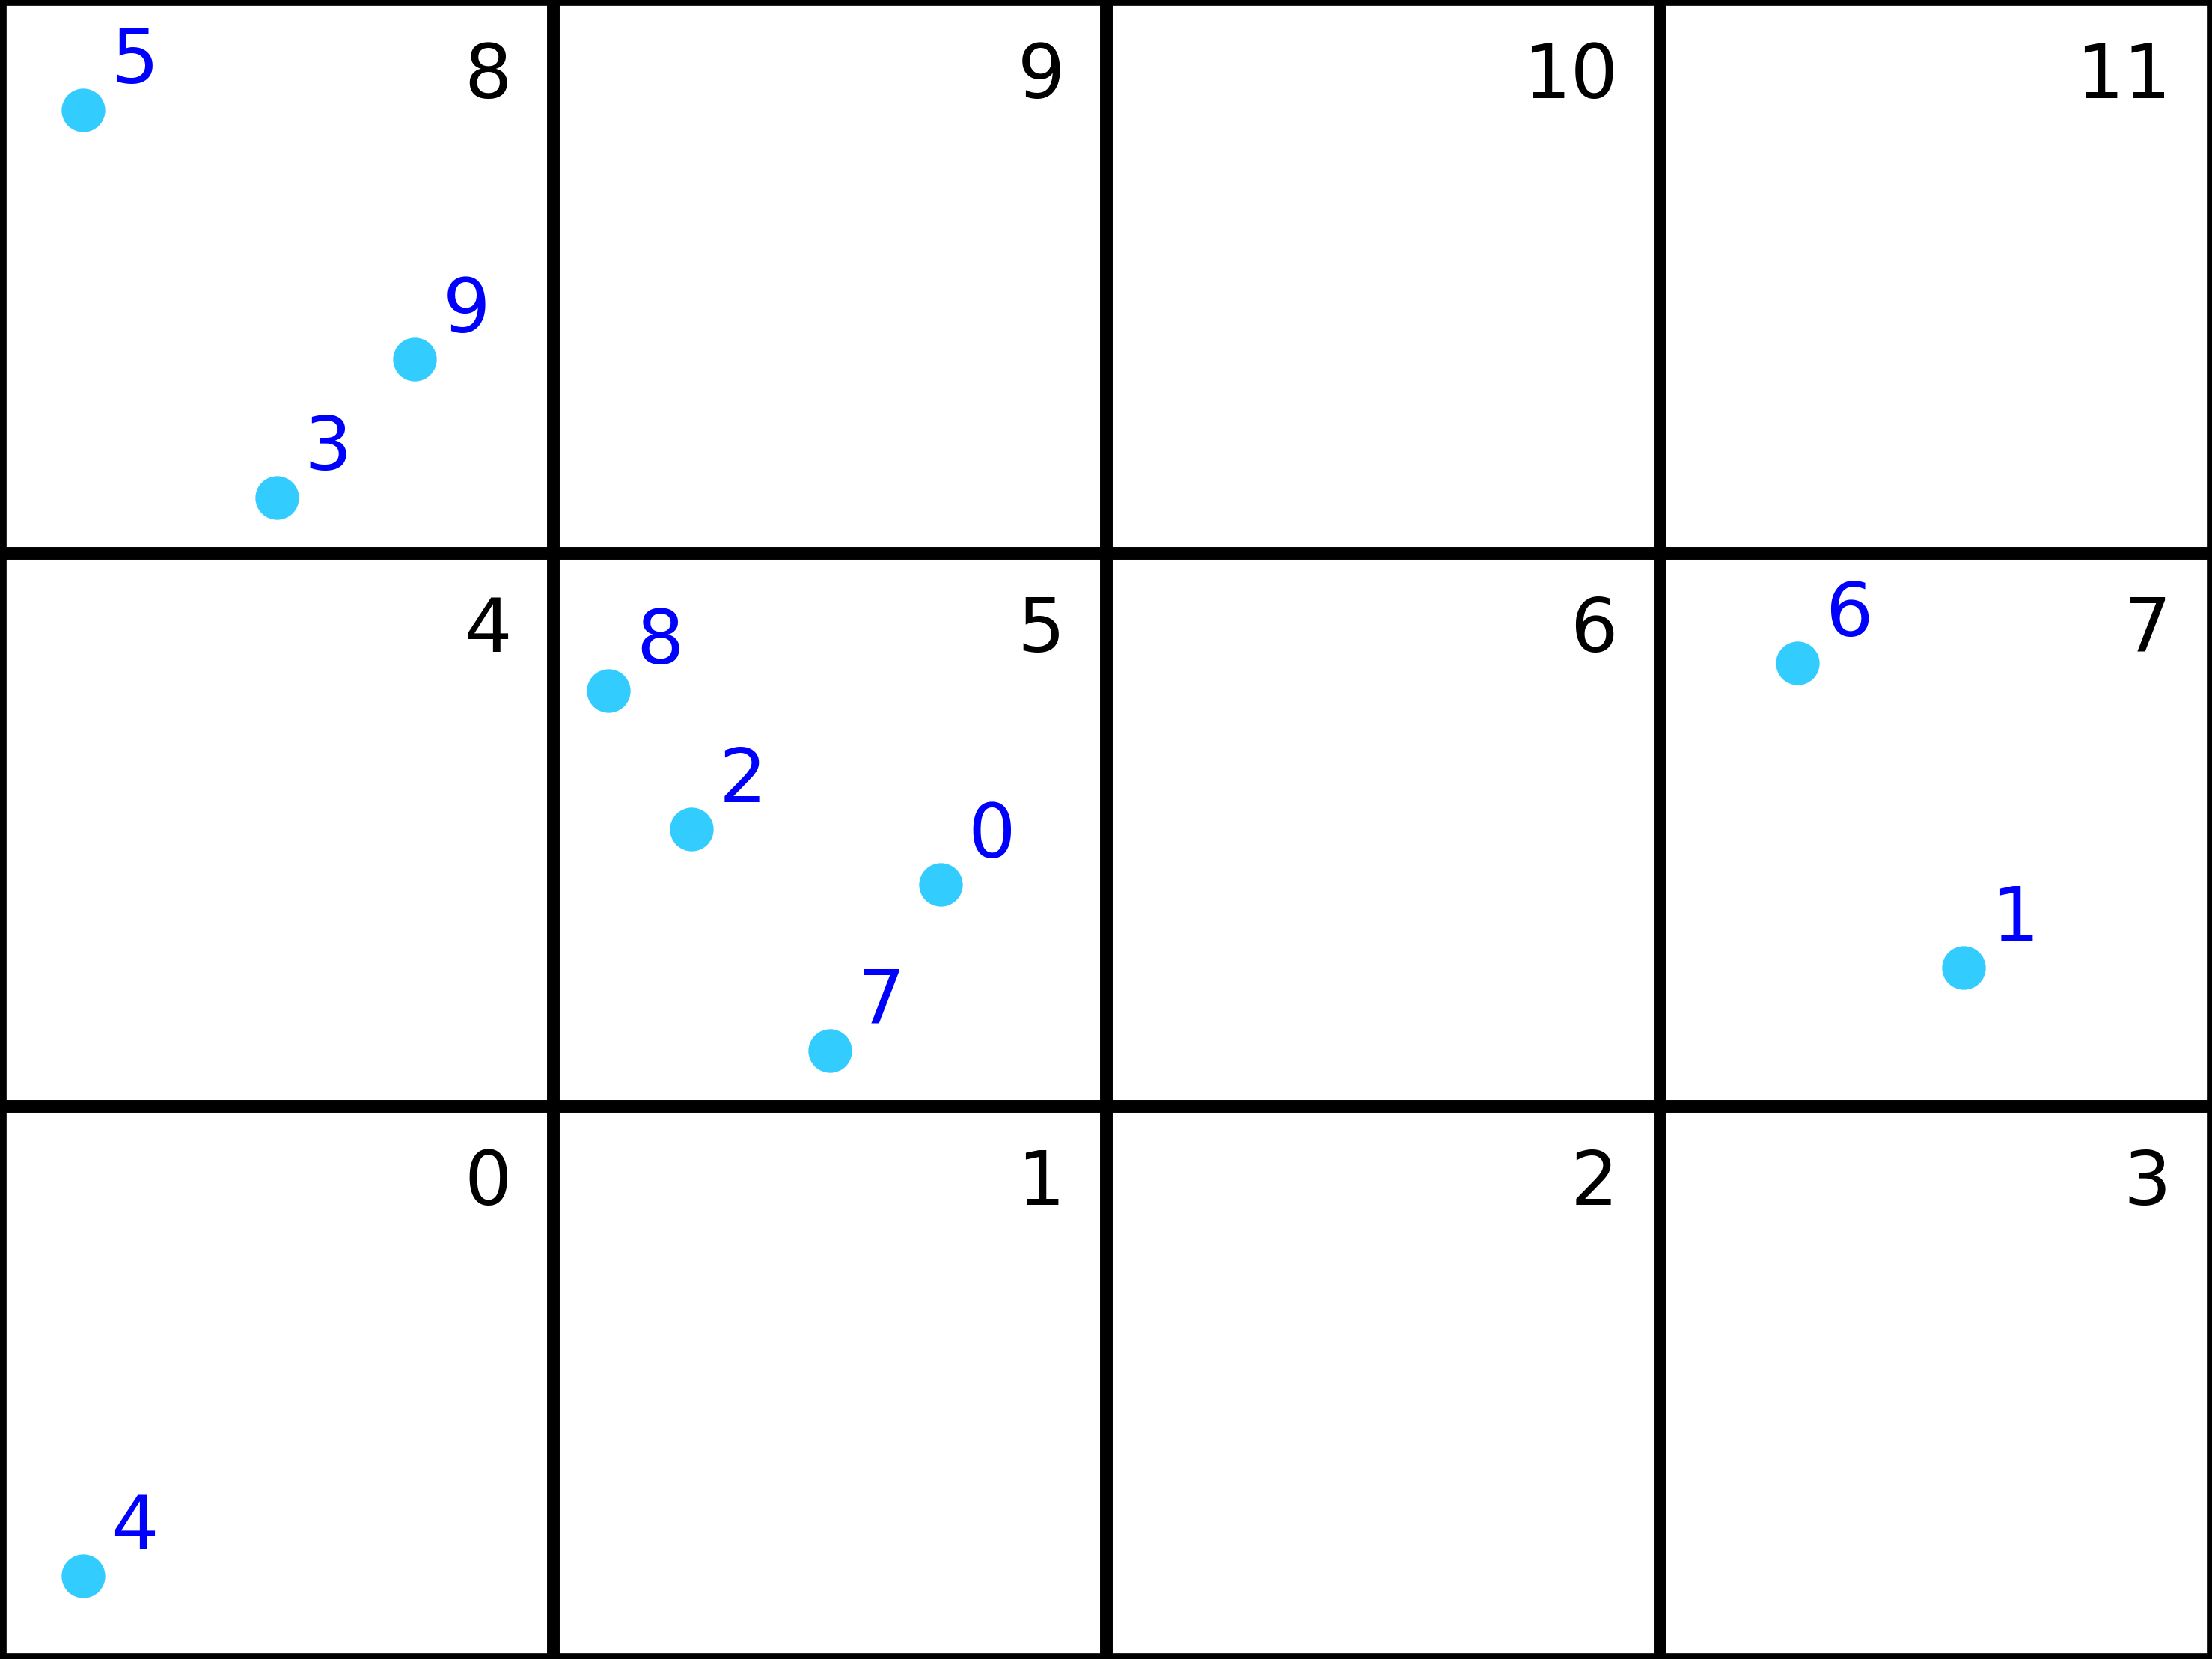
\includegraphics[width=0.4\textwidth]{pictures/grid3.png}
\end{figure}
\end{frame}





\begin{frame}{References}
\begin{columns}
\begin{column}{0.7\textwidth}
\printbibliography
\end{column}
\begin{column}{0.25\textwidth}
\centering
Download this pdf:
\begin{figure}

\includegraphics[width=1\textwidth]{pictures/download.png}
\end{figure}
\end{column}
\end{columns}
\end{frame}





\end{document}
